%%%%%%%%%%%%%%%%%%%%%%%%%%%%%%%%%%%%%%%%%%%%%%%%%%%%%%%%%%%%%%%%%%%%%%%%%%%%%%%
% Uni Duesseldorf
% Lehrstuhl fuer Datenbanken and Informationssysteme
% Vorlage fuer Bachelor-/Masterarbeiten
% Optimiert fuer den Original-Latex-Kompiler LATEX.EXE (LaTeX=>PS=>PDF)
% Version 1.4 - 2.3.2010
%%%%%%%%%%%%%%%%%%%%%%%%%%%%%%%%%%%%%%%%%%%%%%%%%%%%%%%%%%%%%%%%%%%%%%%%%%%%%%%

%%%%%%%%%%%%%%%%%%%%%%%%%%%%%%%%%%%%%%%%%%%%%%%%%%%%%%%%%%%%%%%%%%%%%%%%%%%%%%%
%%%%%%%%%%% BEGINN EINSTELLUNG FUER DIE ARBEIT. UNBEDINGT ERFORDERLICH! %%%%%%%
%%%%%%%%%%%%%%%%%%%%%%%%%%%%%%%%%%%%%%%%%%%%%%%%%%%%%%%%%%%%%%%%%%%%%%%%%%%%%%%
% Geben Sie Ihren Namen hier an
\newcommand{\bearbeiter}{Alina Elterman}

% Geben Sie hier den Titel Ihrer Arbeit an
\newcommand{\titel}{Metrische Dimension Spezieller Graphklassen}

% Geben Sie das Datum des Beginns and Ende der Bachelorarbeit ein
\newcommand{\beginndatum}{28. Juni 2012}
\newcommand{\abgabedatum}{?. Dezember 2012}

% Geben Sie die Namen des Erst- and Zweitgutachters an
\newcommand{\erstgutachter}{Prof. Dr. Egon Wanke}
\newcommand{\zweitgutachter}{PD Dr. Frank Gurski}

% Falls Sie die Arbeit zweiseitig ausdrucken wollen,
% benutzen Sie die folgende Zeile mit
% \AN fuer zweiseitigen Druck
% \AUS fuer einseitigen Druck
\newcommand{\zweiseitig}{\AN}

% Falls die Arbeit in englischer Sprache verfasst 
% werden soll, dann benutzen Sie die folgende Zeile mit
% englisch fuer englische Sprache
% deutsch fuer deutsche Sprache
\newcommand{\sprache}{deutsch}
%%%%%%%%%%%%%%%%%%%%%%%%%%%%%%%%%%%%%%%%%%%%%%%%%%%%%%%%%%%%%%%%%%%%%%%%%%%%%%%%%
%%%%%%%%%%%%%%%%%%%%%%%%%%%%%%% ENDE EINSTELLUNGEN %%%%%%%%%%%%%%%%%%%%%%%%%%%%%%
%%%%%%%%%%%%%%%%%%%%%%%%%%%%%%%%%%%%%%%%%%%%%%%%%%%%%%%%%%%%%%%%%%%%%%%%%%%%%%%%%

% Die folgende Zeile NICHT EDITIEREN oder loeschen
% (Zum Ab�ndern der BA-Vorlage in eine MA-Vorlage muessen sie
% jedoch die Datei titelmakros1.tex selbst editieren.)
%%%%%%%%%%%%%%%%%%%%%%%%%%%%%%%%%%%%%%%%%%%%%%%%%%%%%%%%%%%
% Obere Titelmakros. Editieren Sie diese Datei nur, wenn
% Sie sich ABSOLUT sicher sind, was Sie da tun!!!
% (Z.B. zum Abaendern der BA-Vorlage in eine MA-Vorlage)
% Uni Duesseldorf
% Lehrstuhl fuer Datenbanken und Informationssysteme
% Version 2.2 - 2.3.2010
%%%%%%%%%%%%%%%%%%%%%%%%%%%%%%%%%%%%%%%%%%%%%%%%%%%%%%%%%%%
\newcommand{\AN}{twoside}
\newcommand{\AUS}{}
%\newcommand{\englisch}{}
%\newcommand{\deutsch}{\usepackage[german]{babel}}

%% Die folgenden auskommentierten Optionen dienen der automatischen
%% Erkennung des Latex-Kompilers und dem Setzen der davon abh�ngigen
%% Einstellungen. Bei Problem z.B. mit dem Einbinden von verschiedenen
%% Grafiktypen bei Verwendung von PdfLatex oder Latex, einfach die
%% verschiedenen \usepackage(s) ausprobieren. (Mit diesen Einstellungen
%% funktionierte diese Vorlage bei der Verwenundg von latex.exe als
%% Kompiler bei den meisten Studierenden.)

%\newif\ifpdf \ifx\pdfoutput\undefined
%\pdffalse % we are not running pdflatex
%\else
%\pdfoutput=1 % we are running pdflatex
%\pdfcompresslevel=9 % compression level for text and image;
%\pdftrue \fi[cleardoublepage=plain]

\documentclass[11pt,a4paper,pointlessnumbers, \zweiseitig]{scrreprt}



%\usepackage[iso]{umlaute}
%\usepackage[latin1]{inputenc}
\usepackage{palatino} % palatino Schriftart
%\usepackage{makeidx} % um ein Index zu erstellen
\usepackage{tocbibind}
\usepackage[T1]{fontenc} %fuer richtige Trennung bei Umlauten
\usepackage{fancybox} % fuer die Rahmen
\usepackage{shortvrb}
\usepackage{ifthen}
%\ifthenelse{\equal{\sprache}{deutsch}}{\usepackage[ngerman]{babel}}{}
\usepackage[utf8]{inputenc}
\usepackage[ngerman]{babel}
\usepackage{lmodern} 
\usepackage{amsmath}
\usepackage{oldgerm}
\usepackage{amssymb}
\usepackage{pdfpages}
\usepackage{hyperref}
%\usepackage{fancyheadings}
\usepackage{fancyhdr}
\usepackage{amsfonts}
%\usepackage{complexity}
\usepackage{amsthm}
\usepackage{color}
\usepackage{caption}
%\usepackage{stmaryrd}
\usepackage{graphicx}
\usepackage{graphics}
\usepackage{nomencl}
\usepackage[normalem]{ulem} 
\usepackage{verbatim}
\usepackage{ulsy}
\usepackage{floatflt}
\usepackage{float}
\usepackage{tikz}
\usepackage{pgf}
\usepackage{bbding}
\usepackage{nicefrac}
\usepackage{stmaryrd}
\usepackage{tabularx}
\usepackage{multirow}
\usepackage{array}
\usepackage{algorithm}
\usepackage{algorithmic}
% \usepackage[disable]{todonotes}				% alle todo-Anmerkungen ausblenden
\usepackage[german, color=yellow!40, colorinlistoftodos, textsize=footnotesize, shadow]{todonotes}
\usetikzlibrary{arrows,automata,petri,shapes,snakes}


\newcommand{\markup}[1]{\uline{#1}}
% Befehl umbenennen in abk
\let\abk\nomenclature

\usepackage{a4wide} % ganze A4 Weite verwenden

%\ifpdf
%\usepackage[pdftex,xdvi]{graphicx}
%\usepackage{thumbpdf} %thumbs fuer Pdf
%\usepackage[pdfstartview=FitV]{hyperref} %anklickbares Inhaltsverzeichnis
%\else
%\usepackage[dvips,xdvi]{graphicx}
%\usepackage{hyperref} %anklickbares Inhaltsverzeichnis
%\fi

%%%%%%%%%%%%%%%%%%%%%%% Massangaben fuer die Arbeit %%%%%%%%%%%%%%%
\setlength{\textwidth}{15cm}

\setlength{\oddsidemargin}{35mm}
\setlength{\evensidemargin}{25mm}

\addtolength{\oddsidemargin}{-1in}
\addtolength{\evensidemargin}{-1in}

%\makeindex
% Umgebungen f"ur S�tze usw.
\clearpage{\pagestyle{empty}\cleardoublepage}
\newtheorem{bem}{Bemerkung}
\newtheorem{definition}{Definition}
\newtheorem{bezeichnungen}{Bezeichnungen}
\newtheorem{fakt}{Fakt}
\newtheorem{beispiel}{Beispiel}
\newtheorem{bsp}{Beispiel}
\newtheorem{satz}{Satz}
\newtheorem{lem}{Lemma}
\newtheorem{folg}{Folgerung}
\newtheorem{idee}{Idee}
\newtheorem{corollary}{Korollar}
\floatname{algorithm}{Algorithmus}
\renewcommand{\algorithmicrequire}{\textbf{Eingabe:}}
\renewcommand{\algorithmicensure}{\textbf{Ausgabe:}}
\newenvironment{defi}[1][]{\ifthenelse{\equal{#1}{}}{\definition}{\definition[#1]}\rm}{\enddefinition}
\newcommand{\EP}[3]{
\medskip
\begin{center}
\begin{tabularx}{0.92\textwidth}{ll}
\hline\hline
\multicolumn{2}{c}{\textsc{#1}} \\
\hline
\em{Gegeben:}& #2\\
\em{Frage:}& #3 \\
\hline\hline
\end{tabularx}
\end{center}
\medskip}

\newcommand{\MP}[3]{
\medskip
\begin{center}
\begin{tabularx}{0.92\textwidth}{ll}
\hline\hline
\multicolumn{2}{c}{\textsc{#1}} \\
\hline
\em{Gegeben:}& #2\\
\em{Gesucht:}& #3 \\
\hline\hline
\end{tabularx}
\end{center}
\medskip}

%definition of new commands
\newcommand{\vsp}{\vspace{3mm}}
\newcommand{\impl}[1]{\overset{\text{#1}}{\implies}}
\newcommand{\notimplleft}[1]{\overset{\text{#1}}{\not\Leftarrow}}
\renewcommand{\figurename}{Abbildung}
\renewcommand{\tablename}{Tabelle}
\renewcommand{\contentsname}{Inhaltsverzeichnis}
\renewcommand{\listfigurename}{Abbildungsverzeichnis}
\renewcommand{\listtablename}{Tabellenverzeichnis}
\renewcommand\bibname{Literaturverzeichnis}
\begin{document}

%\setcounter{secnumdepth}{4} %Nummerieren bis in die 4. Ebene
%\setcounter{tocdepth}{4} %Inhaltsverzeichnis bis zur 4. Ebene

\pagestyle{headings}
\thispagestyle{empty}
\sloppy % LaTeX ist dann nicht so streng mit der Silbentrennung
%\MakeShortVerb{\�}

\parindent0mm
\parskip0.5em


{
\textwidth170mm 
\oddsidemargin30mm 
\evensidemargin30mm 
\addtolength{\oddsidemargin}{-1in}
\addtolength{\evensidemargin}{-1in}

\parskip0pt plus2pt

% Die Raender muessen eventuell fuer jeden Drucker individuell eingestellt
% werden. Dazu sind die Werte fuer die Abstaende `\oben' und `\links' zu
% aendern, die von mir auf jeweils 0mm eingestellt wurden.

%\newlength{\links} \setlength{\links}{10mm}  % hier abzuaendern
%\addtolength{\oddsidemargin}{\links}
%\addtolength{\evensidemargin}{\links}

\begin{titlepage}
\vspace*{-1.5cm}
  \raisebox{17mm}{
    \begin{minipage}[t]{70mm}
      \begin{center}
        %\selectlanguage{german}
        {\Large INSTITUT FÜR INFORMATIK\\}
        {\normalsize
          Algorithmen und Datenstrukturen
\\
        }
        \vspace{3mm}
        {\small Universitätsstr. 1 \hspace{5ex} D--40225 Düsseldorf\\}
     \end{center}
    \end{minipage}
  }
  \hfill
  \includegraphics[width=130pt]{HHU_Logo}
  \vspace{14em}

% Titel
  \begin{center}
      	\baselineskip=55pt
    	\textbf{\huge \titel}
  	 	\baselineskip=0 pt
   \end{center}

  %\vspace{7em}

\vfill

% Autor
  \begin{center}
    \textbf{\Large
      \bearbeiter
    }
  \end{center}

  \vspace{35mm}
 
% Pr�fungsordnungs-Angaben
  \begin{center}
    %\selectlanguage{german}
    
%%%%%%%%%%%%%%%%%%%%%%%%%%%%%%%%%%%%%%%%%%%%%%%%%%%%%%%%%%%%%%%%%%%%%%%%%
% Ja, richtig, hier kann die BA-Vorlage zur MA-Vorlage gemacht werden...
%%%%%%%%%%%%%%%%%%%%%%%%%%%%%%%%%%%%%%%%%%%%%%%%%%%%%%%%%%%%%%%%%%%%%%%%%
    {\Large Masterarbeit}

    \vspace{2em}

    \begin{tabular}[t]{ll}
      Beginn der Arbeit:& \beginndatum \\
      Abgabe der Arbeit:& \abgabedatum \\
      Gutachter:         & \erstgutachter \\
                         & \zweitgutachter \\
    \end{tabular}
  \end{center}

\end{titlepage}

}

\thispagestyle{empty}
%%%%%%%%%%%%%%%%%%%%%%%%%%%%%%%%%%%%%%%%%%%%%%%%%%%%%%%%%%%%%%%%%%%%%
%\clearpage
%\begin{titlepage}
%  ~                % eine leere Seite hinter dem Deckblatt
%\end{titlepage}
%%%%%%%%%%%%%%%%%%%%%%%%%%%%%%%%%%%%%%%%%%%%%%%%%%%%%%%%%%%%%%%%%%%%%
\clearpage
~
\newpage
\begin{titlepage}
\vspace*{\fill}

\section*{Erklärung}

%%%%%%%%%%%%%%%%%%%%%%%%%%%%%%%%%%%%%%%%%%%%%%%%%%%%%%%%%%%
% Und hier ebenfalls ggf. BA durch MA ersetzen...
%%%%%%%%%%%%%%%%%%%%%%%%%%%%%%%%%%%%%%%%%%%%%%%%%%%%%%%%%%%

Hiermit versichere ich, dass ich diese Masterarbeit
selbstständig verfasst habe. Ich habe dazu keine anderen als die
angegebenen Quellen und Hilfsmittel verwendet.

\vspace{25 mm}

\begin{tabular}{lc}
Düsseldorf, den \abgabedatum \hspace*{2cm} & \underline{\hspace{6cm}}\\
& \bearbeiter
\end{tabular}

\thispagestyle{empty}
\vspace*{\fill}
\end{titlepage}
~
\thispagestyle{empty}
\newpage
%%%%%%%%%%%%%%%%%%%%%%%%%%%%%%%%%%%%%%%%%%%%%%%%%%%%%%%%%%%%%%%%%%%%%
% Leerseite bei zweiseitigem Druck
%%%%%%%%%%%%%%%%%%%%%%%%%%%%%%%%%%%%%%%%%%%%%%%%%%%%%%%%%%%%%%%%%%%%%

%\ifthenelse{\equal{\zweiseitig}{twoside}}{\clearpage\begin{titlepage}
%~\end{titlepage}}{}

%%%%%%%%%%%%%%%%%%%%%%%%%%%%%%%%%%%%%%%%%%%%%%%%%%%%%%%%%%%%%%%%%%%%%

\thispagestyle{empty}
\clearpage
\begin{titlepage}

\thispagestyle{empty}

%%%%%%%%%%%%%%%%%%%%%%%%%%%%%%%%%%%%%%%%%%%%%%%%%%%%%%%%%%%%%%%%%%%%%%%%%%%%%%%%%
%%%%%%%%%%%%%%%%%%%%%%%%%%%% BEGINN ZUSAMMENFASSUNG %%%%%%%%%%%%%%%%%%%%%%%%%%%%%
%%%%%%%%%%%%%%%%%%%%%%%%%%%%%%%%%%%%%%%%%%%%%%%%%%%%%%%%%%%%%%%%%%%%%%%%%%%%%%%%%
Die metrische Dimension \ldots\\
1 SEITE
%%%%%%%%%%%%%%%%%%%%%%%%%%%%%%%%%%%%%%%%%%%%%%%%%%%%%%%%%%%%%%%%%%%%%%%%%%%%%%%%%
%%%%%%%%%%%%%%%%%%%%%%%%%%%%% ENDE ZUSAMMENFASSUNG %%%%%%%%%%%%%%%%%%%%%%%%%%%%%%
%%%%%%%%%%%%%%%%%%%%%%%%%%%%%%%%%%%%%%%%%%%%%%%%%%%%%%%%%%%%%%%%%%%%%%%%%%%%%%%%%

% Die folgende Zeile NICHT EDITIEREN oder loeschen
%%%%%%%%%%%%%%%%%%%%%%%%%%%%%%%%%%%%%%%%%%%%%%%%
% Untere Titelmakros. Editieren Sie diese Datei nur, wenn Sie sich
% ABSOLUT sicher sind, was Sie da tun!!!
%%%%%%%%%%%%%%%%%%%%%%%%%%%%%%%%%%%%%%%%%%%%%%%
\vspace*{\fill}
\end{titlepage}

%%%%%%%%%%%%%%%%%%%%%%%%%%%%%%%%%%%%%%%%%%%%%%%%%%%%%%%%%%%%%%%%%%%%%
% Leerseite bei zweiseitigem Druck
%%%%%%%%%%%%%%%%%%%%%%%%%%%%%%%%%%%%%%%%%%%%%%%%%%%%%%%%%%%%%%%%%%%%%
%%%%%%%%%%%%%%%%%%%%%%%%%%%%%%%%%%%%%%%%%%%%%%%%%%%%%%%%%%%%%%%%%%%%%
\tableofcontents
\thispagestyle{empty}
%\enlargethispage{\baselineskip}
\clearpage \setcounter{page}{1}
%%%%%%%%%%%%%%%%%%%%%%%%%%%%%%%%%%%%%%%%%%%%%%%%%%%%%%%%%%%%%%%%%%%%%
% Leere Seite, falls Inhaltsverzeichnis mit ungerader Seitenzahl und 
% doppelseitiger Druck
%%%%%%%%%%%%%%%%%%%%%%%%%%%%%%%%%%%%%%%%%%%%%%%%%%%%%%%%%%%%%%%%%%%%%
\ifthenelse{ \( \equal{\zweiseitig}{twoside} \and \not \isodd{\value{page}} \)}
	{\pagebreak \thispagestyle{empty} \cleardoublepage}{\clearpage}



%%%%%%%%%%%%%%%%%%%%%%%%%%%%%%%%%%%%%%%%%%%%%%%%%%%%%%%%%%%%%%%%%%%%%
%%%%%%%%%%%%%%%%%%%%%%%%% BEGINN TEXTTEIL %%%%%%%%%%%%%%%%%%%%%%%%%%%
%%%%%%%%%%%%%%%%%%%%%%%%%%%%%%%%%%%%%%%%%%%%%%%%%%%%%%%%%%%%%%%%%%%%%

\listoftodos


\section{Einführung}
\subsection{Geschichte der Metrischen Dimension}
\pagebreak
%%%%%%%%%%%%%%%%%%%%%%%%%%%%%%%%%%%%%%%%%%%%%%%%%%%%%%%%%%%%%%%%%%%%%%%%%%%%%%%%%%%%%%%%%%%%%%%%%%%%%%%%%%%%%%%%
%%%%%%%%%%%%%%%%%%%%%%%%%%%%%%%%%%%%%%%%%%%%%%%%%%%%%%%%%%%%%%%%%%%%%%%%%%%%%%%%%%%%%%%%%%%%%%%%%%%%%%%%%%%%%%%%
%%%%%%%%%%%%%%%%%%%%%%%%%%%%%%%%%%%%%%%%%%%%%%%%%%%%%%%%%%%%%%%%%%%%%%%%%%%%%%%%%%%%%%%%%%%%%%%%%%%%%%%%%%%%%%%%
\section{Grundbegriffe}
Dieses Kapitel dient als Überblick über Grundlegendes aus der Graphtheorie. Es werden wichtige Begriffe und Zusammenhänge, die in dieser Arbeit benötigt werden definiert und an Beispielen illustriert. Einen tieferen Einblick über diese Thematik verschaffen die Bücher von \cite{} und \cite{}.\\
Die gesammten Operationen werden auf den natürlichen Zahlen durchgeführt, welche als $\mathbb{N}=\{1,2,\ldots\}$ notiert werden.

\textbf{2.1.5. Trennungsknoten und Bifurkatoren}
\begin{floatingfigure}[l]{200pt}
\centering
\includegraphics*[width = 200pt]{bilder/bifurkator.pdf}
\caption{Beispiel für einen Bifurkator}
\label{bild:bifurkator}
\end{floatingfigure}  	 
\vspace{-2mm}
Sei ein Graph $G=(V,E)$ gegeben. Für die Knoten $z,x$ und $y$ besteht die Menge $B$ aus allen Knoten die gleichzeitig auf einem kürzesten Weg von $z$ zu $x$ und auf einem kürzesten Weg von $z$ zu $y$ liegen. Ein Knoten $v$ aus der Menge $B$ mit maximaler Distanz zum Knoten $z$ wird als ein \emph{Bifurkator} von $z, x, y$ bezeichnet.\\
Sind zwei Knoten $u,v$ durch die Entfernung eines Trennungsknotens$x$ in zwei unterschiedlichen Teilgraphen, so liegt der Knoten $x$ auf jedem Wege von $u$ nach $v$.
%%%%%%%%%%%%%%%%%%%%%%%%%%%%%%%%%%%%%%%%%%%%%%%%%%%%%%%%%%%%%%%%%%%%%%%%%%%%%%%%%%%%%%%%%%%%%%%%%%%%%%%%%%%%%%%%
%%%%%%%%%%%%%%%%%%%%%%%%%%%%%%%%%%%%%%%%%%%%%%%%%%%%%%%%%%%%%%%%%%%%%%%%%%%%%%%%%%%%%%%%%%%%%%%%%%%%%%%%%%%%%%%%
%%%%%%%%%%%%%%%%%%%%%%%%%%%%%%%%%%%%%%%%%%%%%%%%%%%%%%%%%%%%%%%%%%%%%%%%%%%%%%%%%%%%%%%%%%%%%%%%%%%%%%%%%%%%%%%%
\section{Eigenschaften der Metrische Dimension}
\subsection{Metrische Dimension von zusammengestellten Graphen}
Betrachte gegebene Graphen mit bekannter Metrische Dimension. Welche Aussagen bezüglich metrischer Dimension lassen sich über unterschiedliche Kompositionen oder Teilgraphen von diesen Graphen formen?\\Dieser Abschnitt widmet sich einerseits der bekannten und bereits erforschten Vereinigung und kartesischen Produkt von zwei Graphen. Andererseits werden zum ersten mal die $r-$fachen Verschmelzung und $r-$fachen Vereinigung von zwei Graphen definiert und Aussagen über ihre metrische Dimension gemacht.\\Bei der Vereinigung und dem kartesischen Produkt werden alle Knoten an der Komposition beteiligt und bei der $r-$fachen Verschmelzung und der $r-$fachen Vereinigung werden die Knoten mit einer Ordnung versehen und zwei gleichmächtige Folgen von Knoten mitübergeben.   
\begin{lem}$\;\;$\\Folgende Schranken gelten für die $r-$fache Verschmelzung von Graphen mit $r \geq 4$:
$$\beta(G_1)+\beta(G_2)-2r \leq \beta(G_1 \infty G_2) \leq \beta(G_1)+\beta(G_2)+r+2 \cdot \lfloor\frac{(r-2)}{3}\rfloor+1$$
\end{lem}

\begin{proof}[Beweis:] 
Um zu zeigen, dass die Schranken strikt sind werden zwei folgende Klassen von Graphen betrachtet. Für die obere Schranke gilt:\\
Betrachte man den folgenden Graphen $G_1$ mit der metrischen Dimension $2$.
\begin{figure}[h!]
		\centering 		 

\includegraphics[width=420pt]{bilder/ver.pdf}
   \caption{Graph $G_1$ mit der metrischen Dimension $2$}
  	 \end{figure}
Um zu zeigen das $\beta(G_1)=2$ betrachte die einzelnen Komponenten des Graphen. Nach Lemma \ref{path} ist bekannt, dass die metrische Dimension eines Weges eins ist. Aufgrund der zwei Blätter am linken und rechten Rand, werden mindestens zwei Knoten in der metrischen Basis benötigt. Auf dem Weg sind zusätzlich Kreise der Größe sechs, aber die Knoten des Graphens werden ohne zusätzlich Vergrößerung der metrischen Dimension getrennt. Betrachte dazu die provisorischen Markierungen in der Abbildung \ref{bild:Kreise}.
\begin{figure}[h!]
		\centering 		 
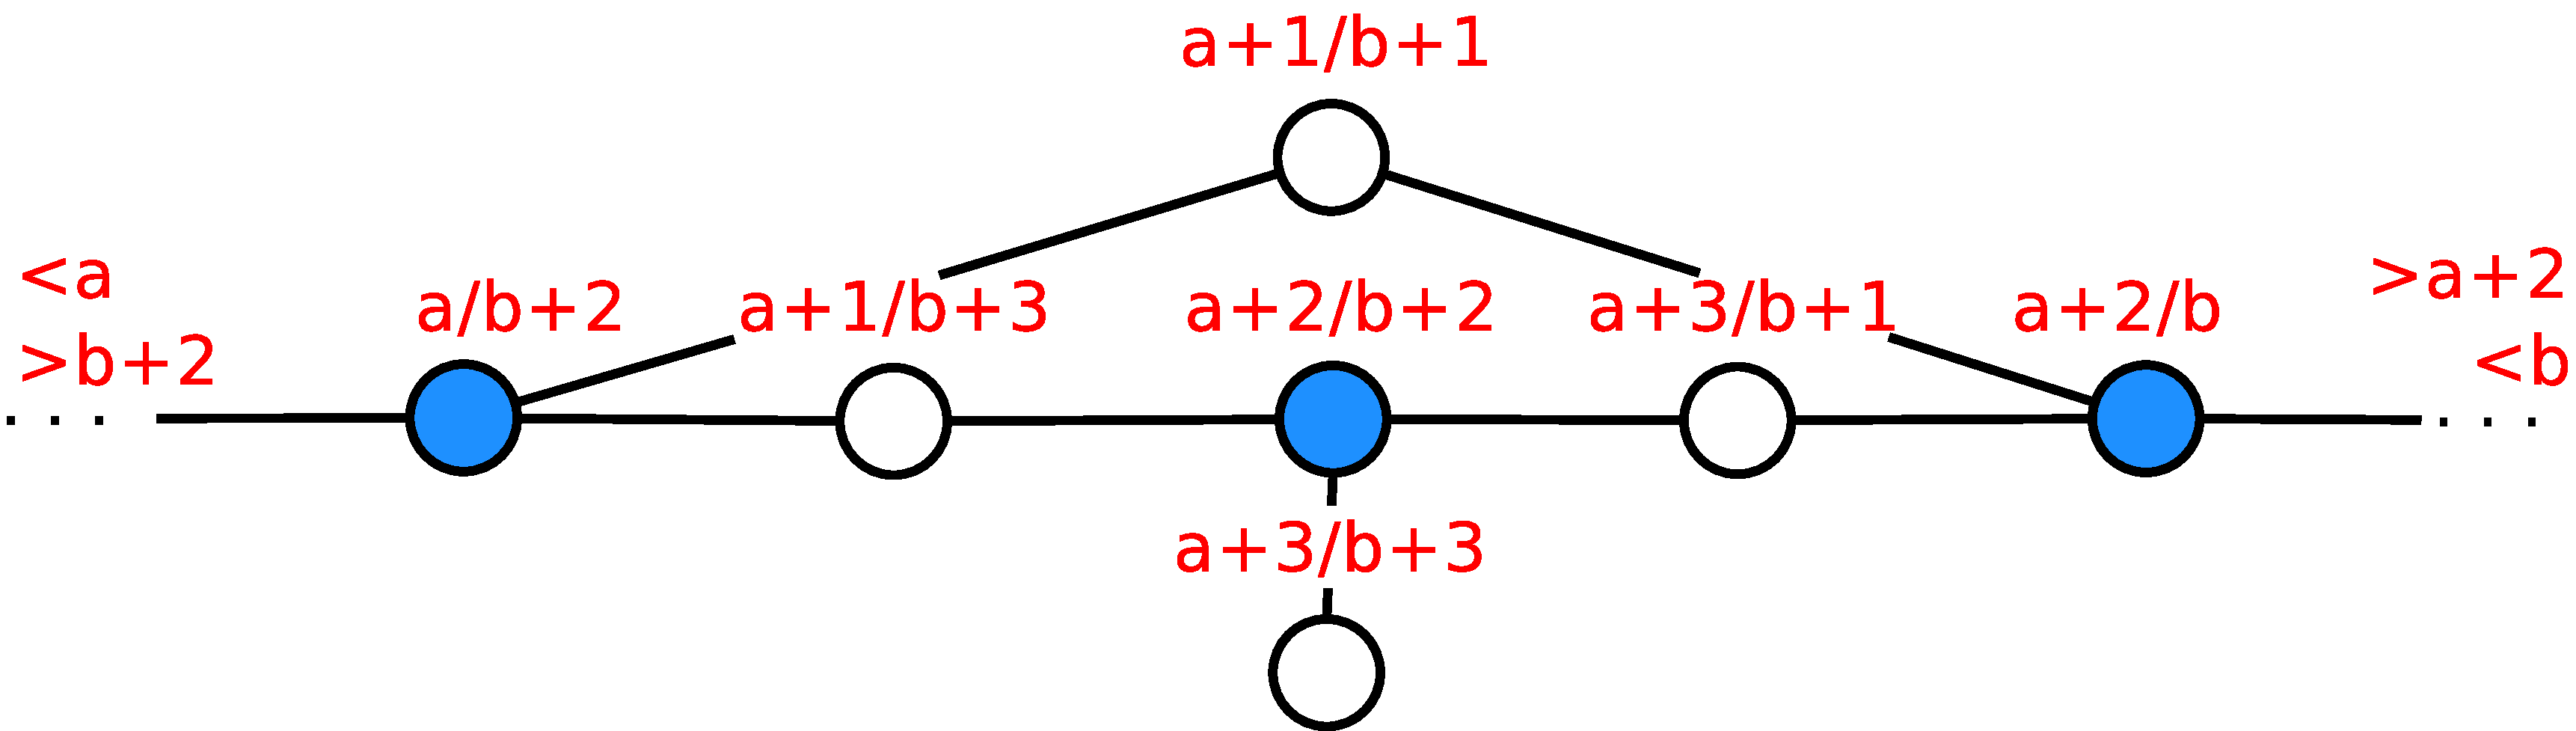
\includegraphics[width=420pt]{bilder/ver2.pdf}
   \caption{Kreise der Länge 6 in Graphen $G_1$}
   \label{bild:Kreise}
  	 \end{figure} 
  	 
Erzeuge einen äquivalenten Graphen $G_2$ mit welchem $G_1$ verschmolzen wird, so entsteht der folgenden Graph:

\begin{figure}[h!]
		\centering 		 

\includegraphics[width=420pt]{bilder/verschmolzenlandmarks.pdf}
   \caption{Graph $G_1$ und $G_2$ wurden verschmolzen}
  	 \end{figure}

Die metrische Dimension von diesem Graphen beträgt:

$$ \beta(G_1)+\beta(G_2)+2+r-1+ \lfloor(r-2)\times\frac{1}{3}\rfloor = \beta(G_1)+\beta(G_2)+r+2 \cdot \lfloor\frac{(r-2)}{3}\rfloor+1$$

\newpage

	   	 
\begin{floatingfigure}[l]{200pt}
\centering
\includegraphics*[width = 160pt]{bilder/gbspver1.pdf}
\caption{Gegenbeispiel für eine mögliche Verbesserung}
\label{bild:aussenknoten}
\end{floatingfigure}
Es nicht möglich dieses Modell durch weitere Kreise zu erweitern. Die außenliegenden Knoten, welche verschmolzen werden, können keine zusätzlichen Kreise bilden, da ein nicht getrenntes Knotenpaar entsteht. Das nichtgetrennte Knotenpaar ist rot markiert in der Abbildung \ref{bild:aussenknoten}. Außerdem muss mindestens ein Knoten, der verschnolzen wird Abstand gehalten werden, ansonsten gibt es mehrere nicht getrennte Knotenpaare, wie in der Abbildung \ref{bild:2hintereinander} dargestellt. Der Versuch weitere größere Kreise zu schaffen, scheitert schon am nächstgrößeren Beispiel, welches in der Abbildung \ref{bild:multikreise} dargestellt ist.

 
 \begin{figure}[h!]
		\centering 		 
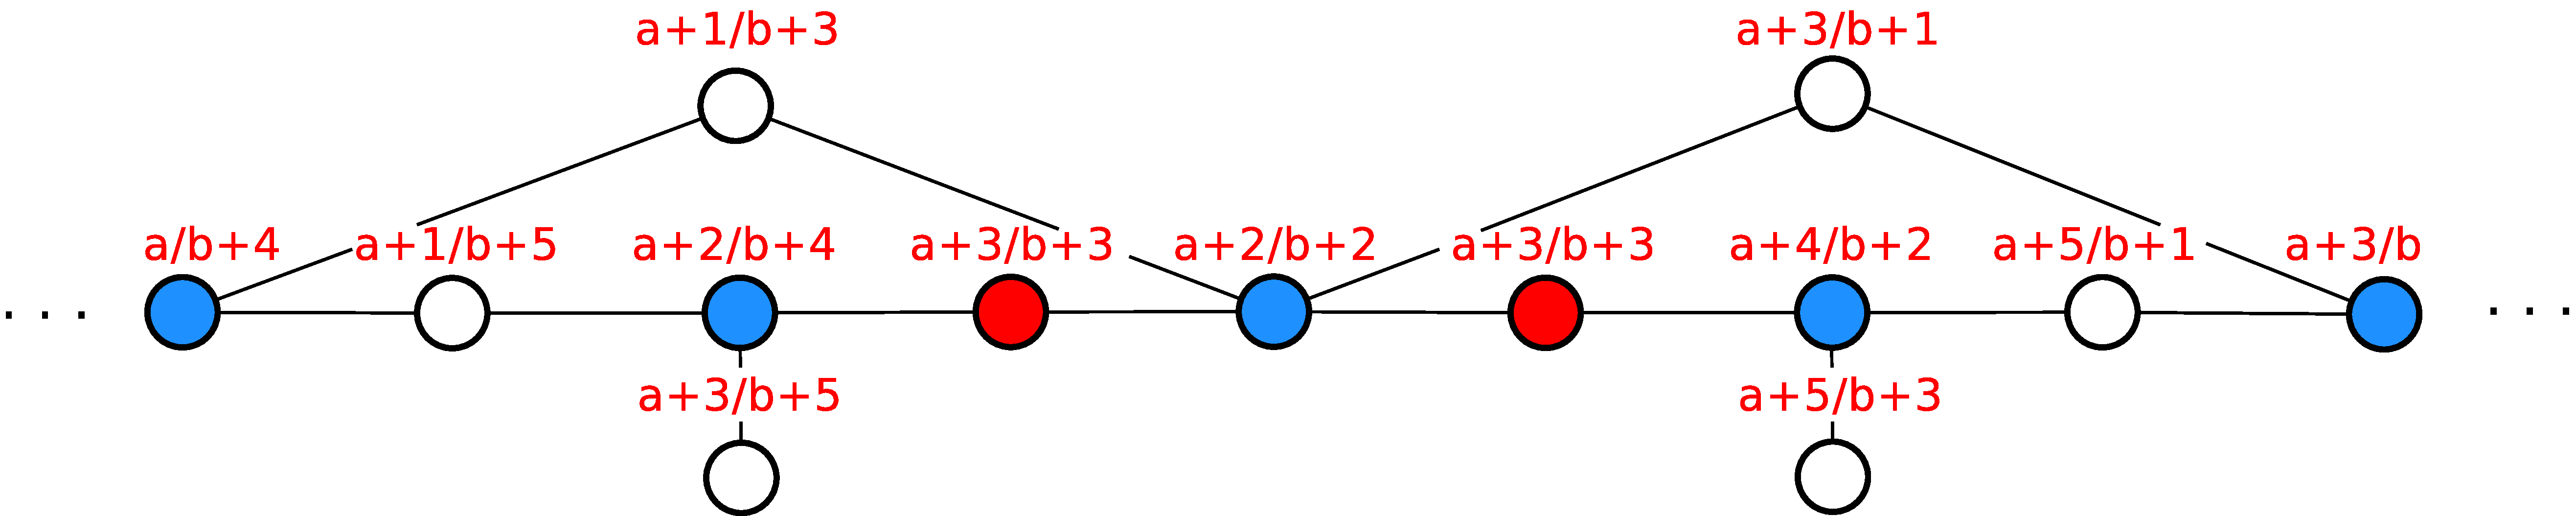
\includegraphics[width=420pt]{bilder/gbspver2.pdf}
   \caption{Gegenbeispiel für eine mögliche Verbesserung}
\label{bild:2hintereinander}  	 
  	 \end{figure}  


 \begin{figure}[h!]
		\centering 		 
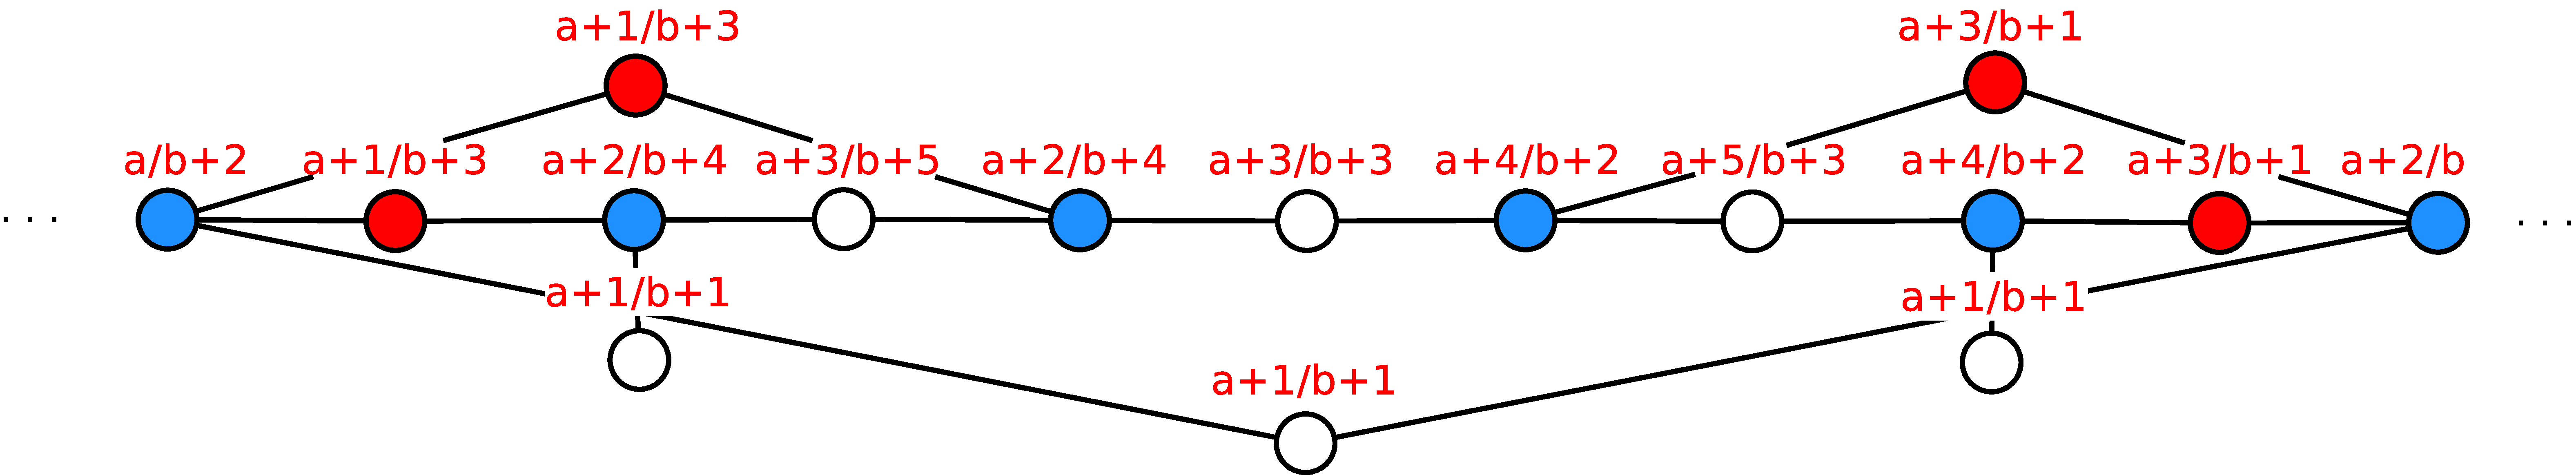
\includegraphics[width=420pt]{bilder/gbsp3.pdf}
   \caption{Gegenbeispiel für eine mögliche Verbesserung}
\label{bild:multikreise}  	 
  	 \end{figure} 
\end{proof}
\subsection{Struktur Eigenschaften}
Es erscheint einem ganz natürlich, dass durch das Entfernen von Kanten sich die metrische Dimension verringert. Nehme man zum Beispiel einen vollständigen Graphen $K_n$ und entferne solange Kanten bis der Graph zu einem einfachen Weg $P_n$ wird. Nun hat sich die metrische Dimension von $n-1$ auf $1$ verringert, also um einen Faktor von $n-1$.\\Interessant ist aber die Eigenschaft, dass durch die Entfernung von Kanten die metrische Dimension auch ansteigen kann. Der folgende Satz und Beweis zeigen, dass sich die metrische Dimension bezüglich des Löschens von Kanten bei einer Graphklasse von einem konstanten Wert um einen unbeschränkten Faktor vergrößert.
\begin{lem}
Die metrische Dimension eines Teilgraphen ist nicht durch die metrische Dimension des ursprünglichen Graphen beschränkt. (Durch das Entfernen von Kanten kann die metrische Dimension eines Graphen steigen.)
\end{lem}
\begin{proof}[Beweis:]$\;$
\begin{figure}[h!]
		\centering 		 
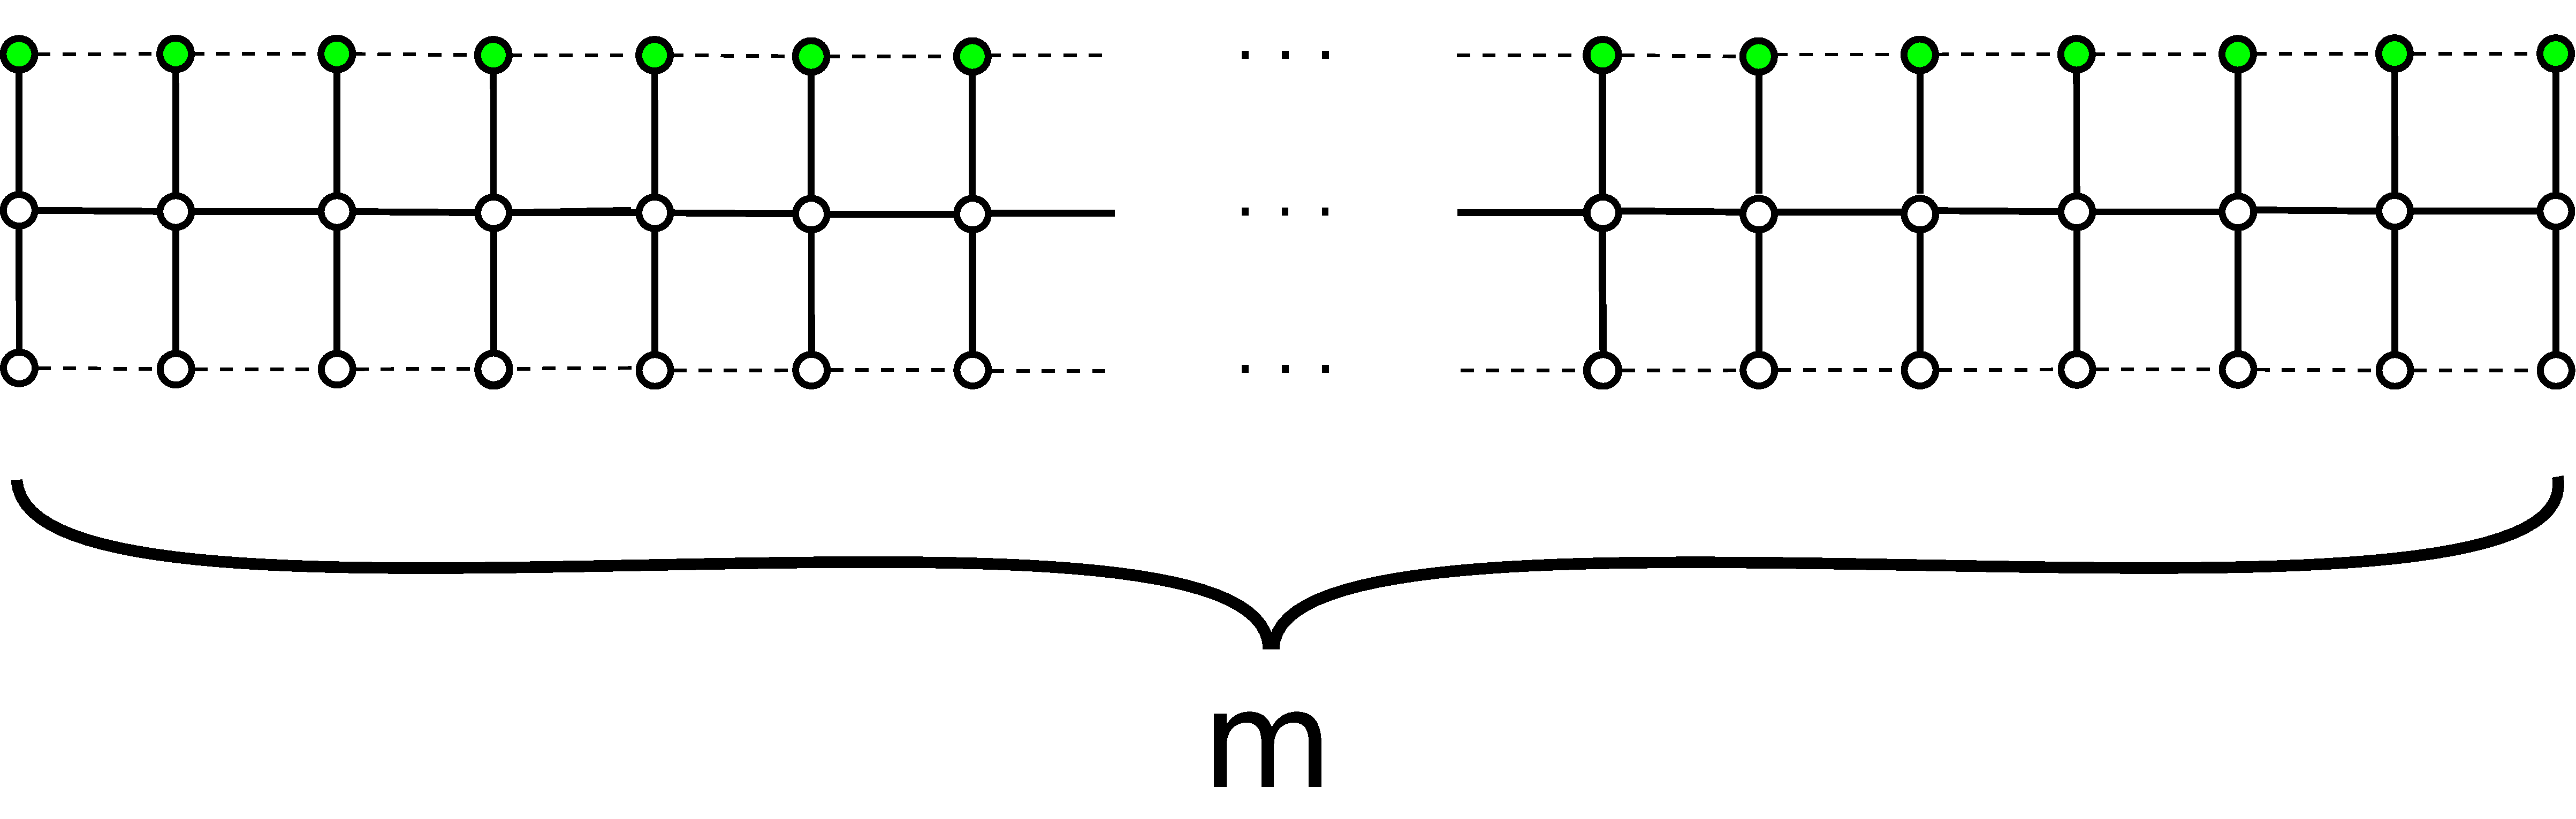
\includegraphics[width=420pt]{bilder/gitterzubaum.pdf}
   \caption{Beispiel für einen Teilgraphen mit größerer MD als der Graph selbst}
   \label{bild:Gitterbaum1}
\end{figure}
\textcolor{white}{x}\newline
Der Gittergraph $G_{3,m}$ hat nach der Tabelle \ref{tbl:Metrische Dimension einiger Graphklassen} metrische Dimension zwei. Entfernt man alle Kanten auf dem aüßeren Kreis so entsteht ein Baum $T_{3m}$ wie in Abbildung \ref{bild:Gitterbaum1} mit der metrischen Dimension $m$. Damit steigt die metrische Dimension von einem Graphen mit $n$ Knoten von zwei auf $\frac{n}{3}$.
\end{proof}
\begin{lem}
Die metrische Dimension eines induzierten Teilgraphen ist nicht durch die metrische Dimension des ursprünglichen Graphen beschränkt. (Durch das Entfernen von Knoten kann die metrische Dimension eines Graphen steigen.)
\end{lem}
\begin{proof}[Beweis:]$\;$
\begin{figure}[h!]
		\centering 		 
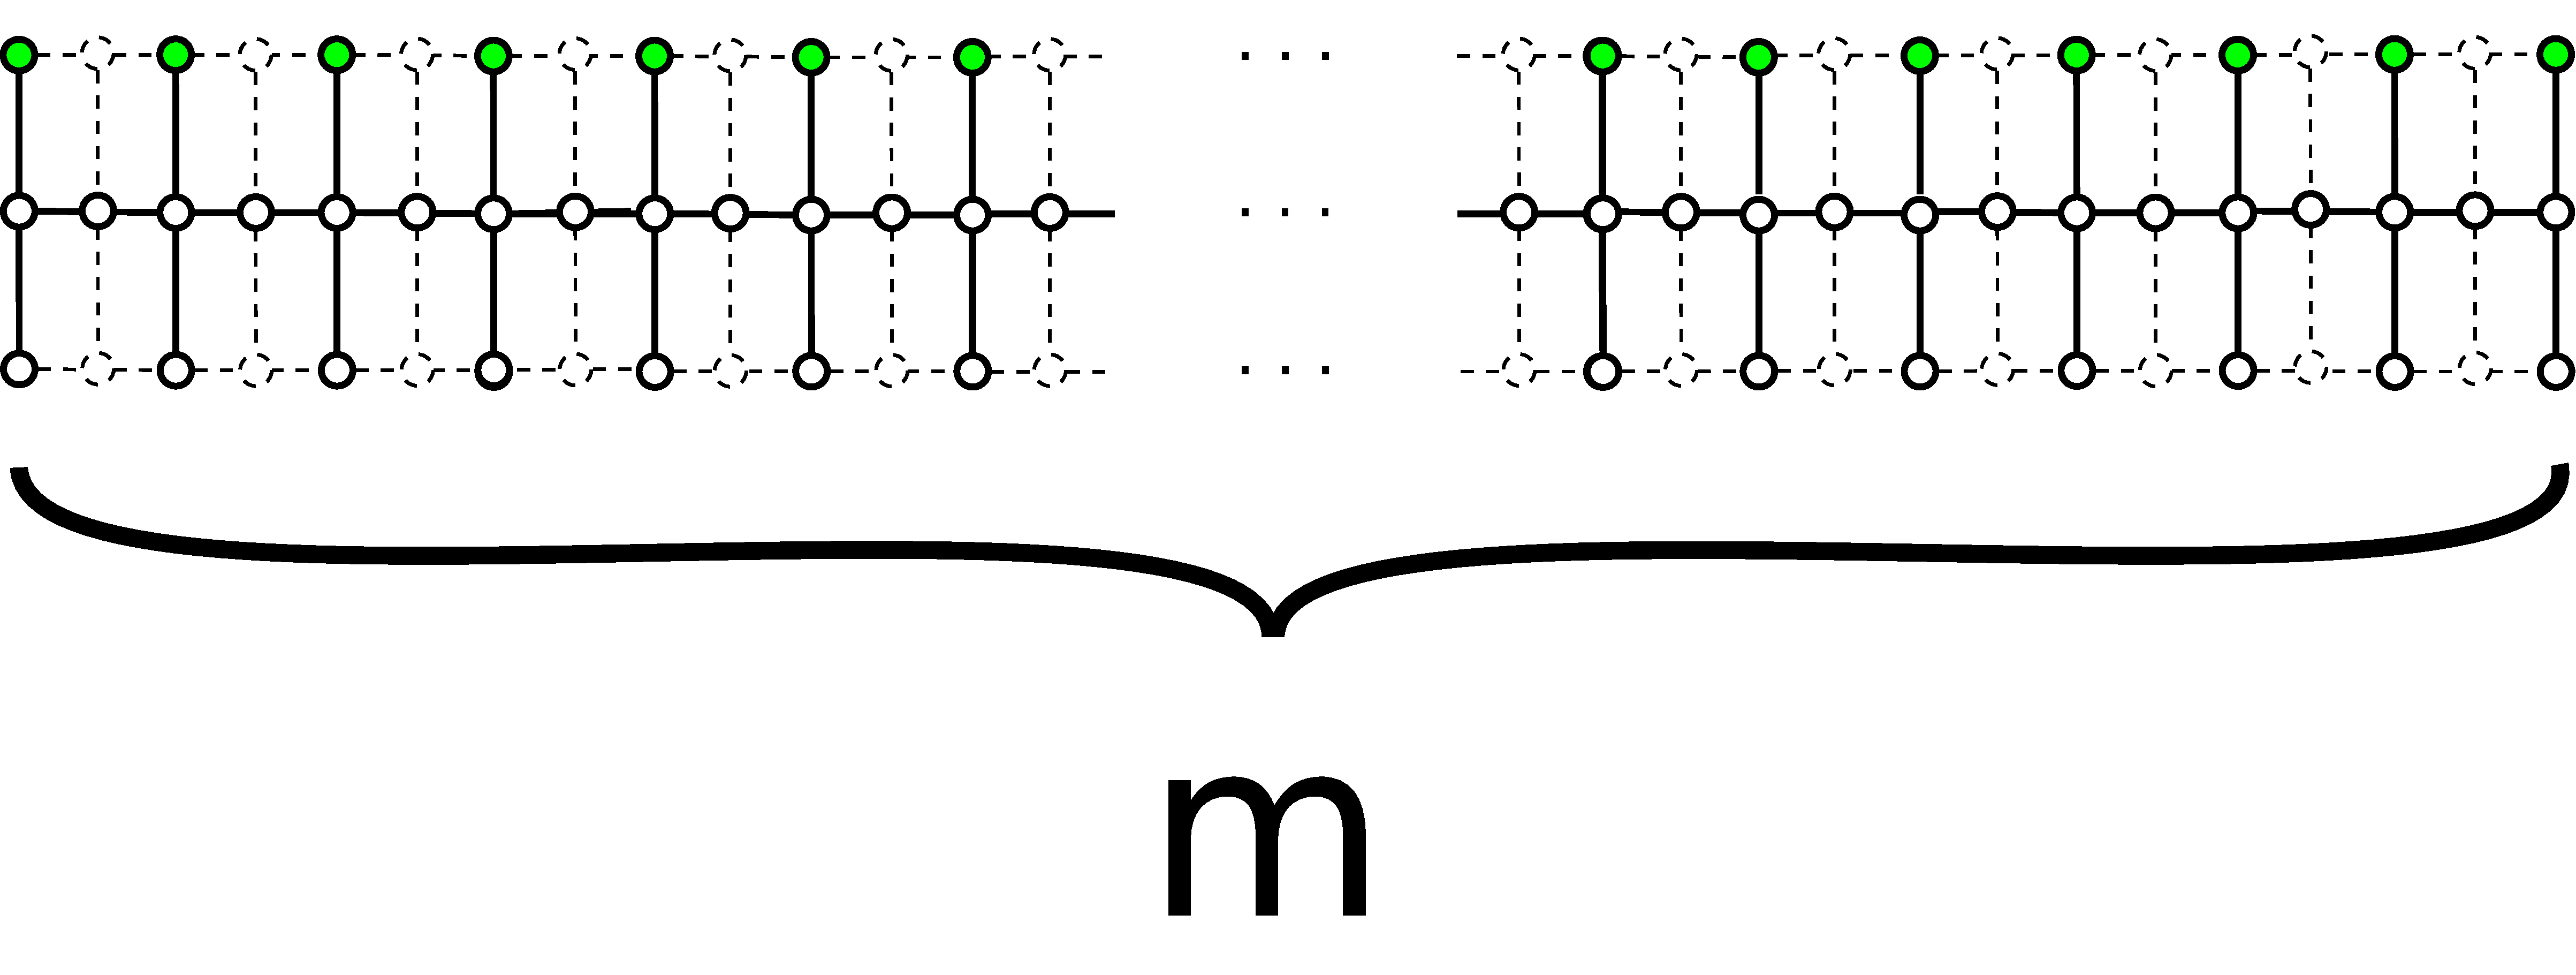
\includegraphics[width=420pt]{bilder/gitterzubaumlsch.pdf}
   \caption{Beispiel für einen induzierten Teilgraphen mit größerer MD als der Graph selbst}
   \label{bild:Gitterbaum2}
  	 \end{figure}
\textcolor{white}{x}\newline
Der Gittergraph $G_{3,2m-1}$ hat nach der Tabelle \ref{tbl:Metrische Dimension einiger Graphklassen} metrische Dimension zwei. Entfernt man jeden zweiten Knoten auf dem aüßeren Kreis so entsteht ein Baum $T_{3m}$ wie in Abbildung \ref{bild:Gitterbaum2} mit der metrischen Dimension $m$. Damit steigt der Anteil von Knoten : Knoten in der metrischen Basis von $6m-3:2$ auf $3m:m$.
\end{proof}
\todo{Entfernen 1ner Kante, 1nem Knoten}\newpage
\begin{lem}
\label{trennungsknoten}
Sei ein beliebiger Graph $G=(V,E)$ gegeben. Seien $G_1$ und $G_2$ zwei disjunkte Teilgraphen von $G$ die durch das Löschen von einem Knoten $x$ entstehen. Jedes Knotenpaar aus $G_2$, welches von einem Knoten aus $G_1$ getrennt wird, wird auch von dem Knoten $x$ getrennt. Es gilt dasselbe für die Knotenpaare in $G_1$.
\end{lem}
\begin{lem}
\label{wegtrennungsknoten}
Sei ein Graph $G=(V,E)$ mit zwei verbundenen Knoten $v_i$ und $v_j$. Es gilt ausserdem $deg(v_j)=2$ und $v_i$ ist ein Trennungsknoten, sodass der Teilgraph mit dem Knoten $v_j$ ein Weg ist. Beinhalte 
\end{lem}
\begin{proof}[Beweis:]
Angenommen $R$ sei eine metrische Basis des Graphen $G$ und der Knoten $v$ besitze die Markierung $a_1/\ldots /a_n$. Sei die $dist_G(v,x)=b$, da $v$ der Bifurkator ist liegt er auf einem kürzesten Weg und so ist die Markierung vom Knoten $x$ $a_1+b/\ldots /a_n+b$. Nach der Vorraussetzung ist $dist_G(v,x)=dist_G(v,y)$, damit hat der Knoten $y$ die Markierung $a_1+b/\ldots /a_n+b$ und die Knoten $x$ und $y$ sind nicht getrennt. Dies ist ein Widerspruch zur Definition der metrischen Basis. $\lightning$
\end{proof}
\begin{lem}
\label{einelementreichtnicht}
Sei ein beliebiger Graph $G=(V,E)$ gegeben. Seien drei Knoten $v_1$, $v_2$ und $v_3$ gegeben, welche jeweils mit dem Knoten $v_4$ verbunden sind und es gilt,dasses paarweise keinen Weg ungerader Länge zwischen zwei von diesen Knoten gibt. Sind die Markierungen von $v_1$, $v_2$ und $v_3$ gleich so reicht die Aufnahme von einem Knoten in die metrische Basis nicht aus um diese Knoten zu trennen.
\end{lem}
\clearpage
%%%%%%%%%%%%%%%%%%%%%%%%%%%%%%%%%%%%%%%%%%%%%%%%%%%%%%%%%%%%%%%%%%%%%%%%%%%%%%%%%%%%%%%%%%%%%%%%%%%%%%%%%%%%%%%%
%%%%%%%%%%%%%%%%%%%%%%%%%%%%%%%%%%%%%%%%%%%%%%%%%%%%%%%%%%%%%%%%%%%%%%%%%%%%%%%%%%%%%%%%%%%%%%%%%%%%%%%%%%%%%%%%
%%%%%%%%%%%%%%%%%%%%%%%%%%%%%%%%%%%%%%%%%%%%%%%%%%%%%%%%%%%%%%%%%%%%%%%%%%%%%%%%%%%%%%%%%%%%%%%%%%%%%%%%%%%%%%%%
\section{Metrische Dimension von kreisähnlichen Graphklassen}
\subsection{Kreis- und Rad-ähnliche Graphklassen}
In diesem Kapitel geht es um Graphen welche Erweiterungen von bereits bekannten und erforschten Graphklassen sind mit festeroder parameterabhängiger metrischer Dimension. Es werden der Freundschaftsgraph und seine Verallgemeinerung, der Sonnengraph, der Helmgraph, der Sonnenblumengraph, der Gear und der Webgraph, sowie eine Erweiterung vom Rad und vom Gittergraphen untersucht.
Von dem Sonnengraphen, sowie bei seiner unvollständigen Variante wird die Dimension berechnet, da diese bei dem Beweis der metrischen Dimension der $C_j-$Bäume benötigt wird.
\subsection{Metrische Dimension von den Freundschaftsgraphen $F_{n}$}
''Haben je zwei Bekannte einen weiteren gemeinsamen Bekannten, so gibt es eine Person, welche alle Anderen kennt''. Diese Behauptung kann durch als ein Graphenproblem definiert werden, wobei Knoten Personen und Kanten Bekannschaften repräsentieren.  Dieser von Paul Erdős etc. in \cite{Erdos} eingeführte Graph wird als Freundschaftsgraph bezeichnet. In dem Paper von Imran etc. wird die Partitionsdimension der Freundschaftsgraphen bestimmt und in diesem Kapitel seine metrische Dimension.
\begin{defi}{\textbf{(Freundschaftsgraph $F_{n,3}$)}}\\
\emph{Seien $n$ Kreise $C_3$ mit der Knotenfolge $|V|=\{v_1,v_2,v_3\}$ gegeben. Durch das Verschmelzen von allen Knoten, welche mit $v_1$ gekenntzeichnet sind entsteht der Freundschaftsgraph $F_{n,3}$. Dieser Graph hat die Ordnung $2n+1$ und die Größe $3n$.}
\end{defi}
\begin{bsp}\textcolor{white}{lala}
\begin{figure}[h!]
\centering
 		 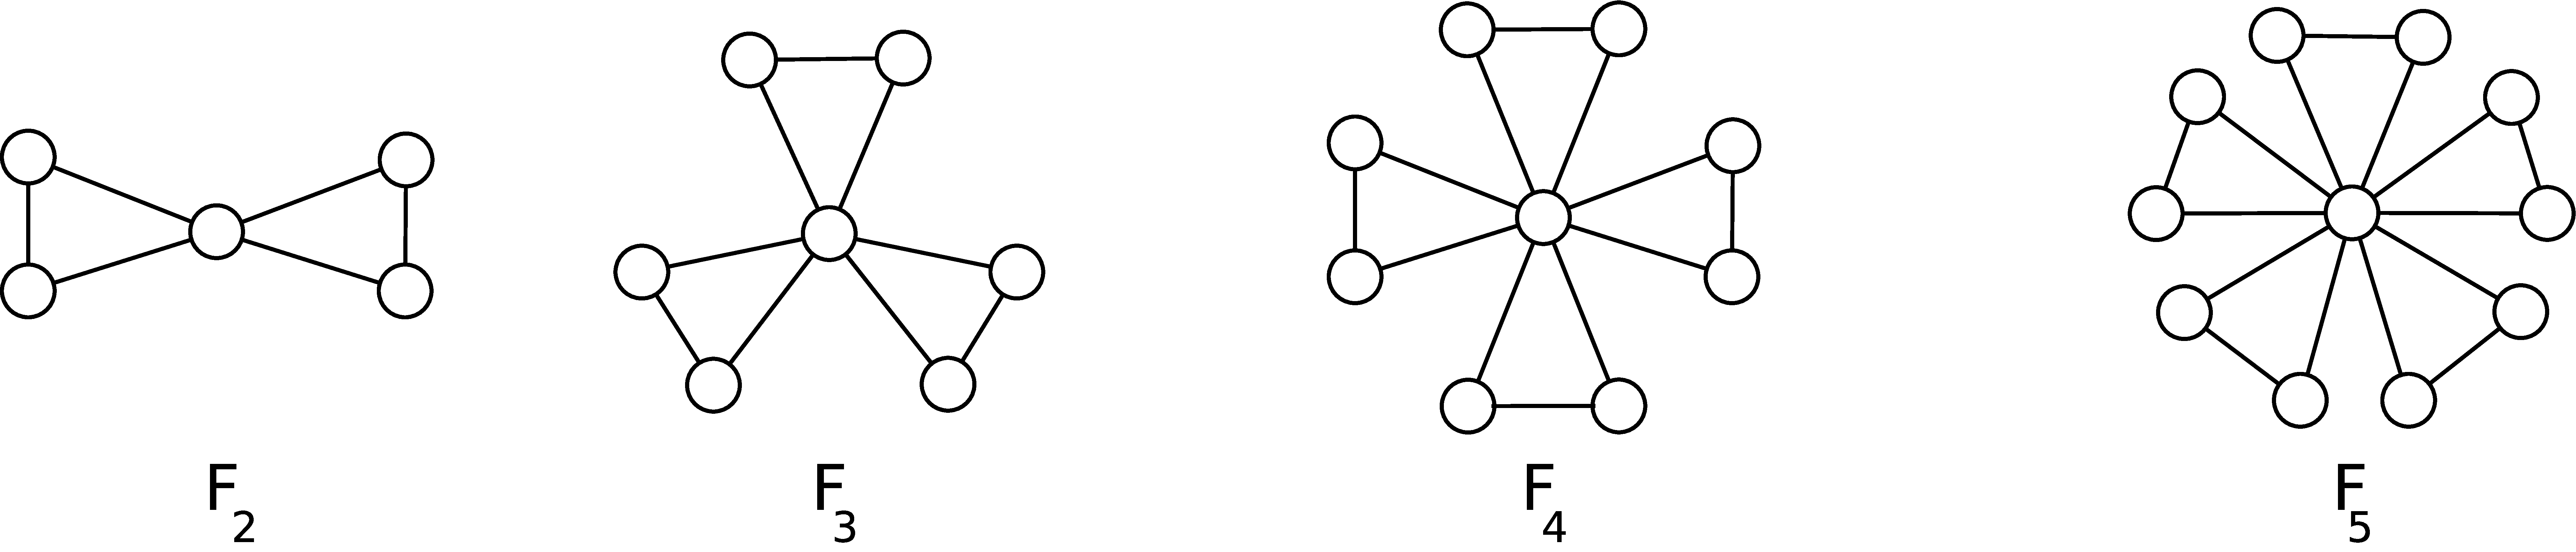
\includegraphics[width=428pt]{bilder/freunschaftsgraph.pdf}
   \caption{Vier Freundschaftsgraphen}
   \label{bild:fg}
\end{figure}
\end{bsp}
\begin{lem}
\label{Freundschaftsgraphen}
Die metrische Dimension eines Freundschaftsgraphen $F_{n,3}$ ist $n$.
\end{lem}
\vspace{-1mm}
Um diese Behauptung zu beweisen, wird das folgende Lemma benötigt. 
\begin{lem}
\label{mindfreundschaftsgraph}
Sei ein Freundschaftsgraph $F_{n,3}$ gegeben. Jede metrische Basis muss aus jedem $C_3$ mindestens einen der folgenden Knoten $\{v_{2},v_{3}\}$ beinhalten.
\end{lem}
\newpage
\begin{proof}[Beweis:]
\textcolor{white}{lala}
\begin{floatingfigure}[l]{230pt}
\centering
\includegraphics*[width = 100pt]{bilder/freundschaftsgraphbew.pdf}
\caption{Ein markierter $C_{3}$}
\end{floatingfigure}
Angenommen es gibt einen $C_3$\\bei welchem keiner dieser Knoten\\in der metrischen Basis ist.\\Durch die eindeutige Verbindung zu dem Restgraphen, welche über  einen\\Trennungsknoten läuft, folgt aus\\Symmetriegründen, dass die Knoten $v_{2}$\\und $v_{3}$ identische Markierungen haben.\\Dies ist ein Widerspruch zu der Definition einer metrischen Basis.\\
Damit ist die metrische Dimension eines Freundschaftsgraphen $F_{n,3}$\\mindestens gleich der Anzahl seiner $C_{3}$ und damit mindestens $n$.\textcolor{white}{lala}\\\textcolor{white}{lala}
\end{proof}
\vspace{-6mm}
\begin{proof}[Beweis von Lemma \ref{Freundschaftsgraphen}:] \vspace{+1mm}
\textcolor{white}{lala}\\ 
Nach Lemma \ref{mindfreundschaftsgraph} ist bekannt, dass die metrische Dimension eines Freundschaftsgraphen $F_n$ mindestens $n$ ist. Angenommen alle als $v_2$ markierten Knoten werden in die metrische Basis aufgenommen, damit sind sie getrennt. Der Knoten $v_1$ hat die Distanz eins zu allen Knoten in der metrischen Basis und ist der einzige Knoten mit dieser Eigenschaft. Für jeden Knoten $v_3$ gibt es genau einen Knoten $v_2$ mit der Distanz eins. Zu allen anderen Knoten in der metrischen Basis hat jeder Knoten $v_3$ die Distanz zwei. Alle Markierungen sind eindeutig und der gesammte Graph ist durch die $n$ Knoten getrennt.
\end{proof}
\vspace{-10mm}
\textcolor{white}{x}\\

Werden nicht nur Kreise der Länge drei sondern beliebiger Länge betrachtet bleibt dennoch ihre metrische Dimesnion $k$ für $k\geq 4$ erhalten.
\begin{defi}{\textbf{(Verallgemeinerter Freundschaftsgraph $F_{n,k}$)}}\\
\emph{Seien $n$ Kreise $C_k=(V_k,E_k)$ mit der Knotenfolge $|V_k|=\{v_1,\ldots,v_k\}$ gegeben. Durch das Verschmelzen von allen Knoten, welche mit $v_1$ gekenntzeichnet sind entsteht der Freundschaftsgraph $F_{n,k}$. Dieser Graph hat die Ordnung $kn+1$ und die Größe $kn$.}
\end{defi}

\begin{lem}
\label{verallgFreundschaftsgraphen}
Die metrische Dimension eines Freundschaftsgraphen $F_{n,k}$ mit $k=2j+1$ für $j \geq 1$ ist $n$ und die metrische Dimension eines Freundschaftsgraphen $F_{n,k}$ mit $k=2j$ für $j \geq 2$ ist $2n-1$.
\end{lem}
\vspace{-1mm}
Um diese Behauptung zu beweisen, wird das folgende Lemma benötigt. 
\begin{lem}
\label{mindverallgfreundschaftsgraph}
Sei ein Freundschaftsgraph $F_{n,k}$ gegeben. Jede metrische Basis muss aus jedem $C_k$ mindestens einen der folgenden Knoten $\{v_{2},\ldots,v_k\}$ beinhalten.
\end{lem}
\begin{proof}[Beweis:]
Angenommen es gibt einen Kreis $C_k$ bei welchem keiner dieser Knoten in der metrischen Basis ist. Durch die eindeutige Verbindung zu dem Restgraphen, welche über einen Trennungsknoten läuft, folgt aus Symmetriegründen, dass die Knoten $v_{2}$ und $v_{k}$ identische Markierungen haben.\\Dies ist ein Widerspruch zu der Definition einer metrischen Basis.\\
Damit ist die metrische Dimension eines Freundschaftsgraphen $F_n$ mindestens gleich der Anzahl seiner $C_{k}$ und damit mindestens $n$.
\end{proof}
\vspace{-6mm}
\begin{proof}[Beweis von Lemma \ref{verallgFreundschaftsgraphen} für $k=2j+1$:] \vspace{+1mm}
\textcolor{white}{lala}\\ 
Nach Lemma \ref{mindverallgfreundschaftsgraph} ist bekannt, dass die metrische Dimension eines Freundschaftsgraphen $F_{n,k}$ mindestens $n$ ist. Angenommen alle als $v_{\lceil \frac{n}{2} \rceil}$ markierten Knoten werden in die metrische Basis aufgenommen, damit sind sie getrennt. Jeder Knoten $v_i$ auf dem jeweiligen Kreis hat die Distanz $\leq \lfloor \frac{n}{2} \rfloor$ zu dem Knoten $v_{\lceil \frac{n}{2} \rceil}$ und die Distanz $\geq \lfloor \frac{n}{2} \rfloor$ zu allen Knoten in der metrischen Basis. Der Knoten $v_1$ hat als einziger Knoten die Distanz $\lfloor \frac{n}{2} \rfloor$ zu allen Anderen. Jeder andere Knoten ist nach den Sätzen \ref{tbl:Metrische Dimension einiger Graphklassen} und \ref{} getrennt.
\end{proof}
\begin{proof}[Beweis von Lemma \ref{verallgFreundschaftsgraphen} für $k=2j$:] \vspace{+1mm}
\textcolor{white}{lala}\\ 
Nach Lemma \ref{mindverallgfreundschaftsgraph} ist bekannt, dass die metrische Dimension eines Freundschaftsgraphen $F_{n,k}$ mindestens $n$ ist. \todo{Beweis auschreiben}
\end{proof}
\begin{lem}
Die metrische Dimension von allgemeinen Freundschaftgraphen $F_{n}$ mit unterschiedlicher Kreislänge ist $n+n_g-1$. Dabei ist $n=n_u+n_g$ und $n_u$ ist die Anzahl der Kreise mit ungerader Länge und $n_g$ die Anzahl der Kreise mit gerader Länge.
\end{lem}
\newpage
%%%%%%%%%%%%%%%%%%%%%%%%%%%%%%%%%%%%%%%%%%%%%%%%%%%%%%%%%%%%%%%%%%%%%%%%%%%%%%%%%%%%%%%%%%%%%%%%%%%%%%%%%%%%%%%%
\subsection{Metrische Dimension von den Sonnengraphen $S_{n,k}$}
In dem breiten Spektrum an Literatur über die metrische Dimension hat sich niemand bis jetzt für die metrische Dimension von dieser Graphklasse interessiert. Dennoch gibt es Ergebnisse über einen Spezialfall und zwar den Drachengraphen \cite{blabla}, wo ein Kreis mit einem Weg durch eine Kante an einen Endknoten des Weges vereinigt wird, seine metrische Dimension ist zwei.

\begin{defi}{\textbf{(Sonnengraph $S_{n,k}$)}}\\
\emph{Sei ein Kreis $C_n$ für $n \geq 3$ mit der Knotenmenge $|V|=\{ c_1, \ldots , c_n \}$ und $n$ Weggraphen $P_{k-1}$ für $k\geq 2$ gegeben.\\Die Knoten mit Grad eins auf dem $i-$ten Weg werden als $v_{i,1}$ und $v_{i,k-1}$ bezeichnet. Durch das Hinzufügen von $n$ neuen Kanten der Form $\{v_{i,1},c_i\}$ für $1 \leq i \leq n$ ensteht der zusammenhängende Sonnengraph $S_{n,k}$.\\
Alle als $v_{i,k-1}$ bezeichneten Knoten werden Endknoten genannt, als $c_i$ bezeichneten Knoten werden Ursprungsknoten genannt und eine Knotenmenge mit den\\Knoten $\{c_i,v_{i,1}, \ldots ,v_{i,k-1}\}$ für $1 \leq i \leq n$ als Strahl. (vgl. Abbildung \ref{bild:sonnengraph})\\
Für $n=1$ ist der Graph der Sterngraph aus Definition \ref{defstern}.}
\end{defi}
\begin{figure}[h!]
\centering
 		 \includegraphics[width=165pt]{bilder/sonne4.pdf}
   \caption{Der Sonnengraph $S_{12,3}$}
   \label{bild:sonnengraph}
\end{figure}
\begin{lem}
Die metrische Dimension eines Sonnengraphen $S_{n,k}$ mit $n = 2j+1$ für $j \in \mathbb{N}$ und $k \geq 1$ ist zwei und die metrische Dimension eines Sonnengraphen $S_{n,k}$ mit $n = 2j+4$ für $j \in \mathbb{N}$ und $k \geq 1$ ist drei. 
\end{lem}

\begin{lem}
Die metrische Dimension eines Sonnengraphen $S_{n,k}$ mit $n = 2j+4$ für $j \in \mathbb{N}$ und $k \geq 1$ kann nicht zwei sein. 
\end{lem}
\begin{proof}[Beweis:]
Für den ersten Knoten in der metrischen Basis gibt es $(k-1)\cdot n$ Möglichkeiten, aber nur $n$ unterschiedliche Fälle. Denn wird der erste Knoten aus einem Strahl aufgenommen, so gilt nach Lemma \ref{} das der Strahlursprung als Element der metrischen Basis betrachtet werden kann. Der zweite Knoten muss die Bedingung vom Lemma \ref{Bifurnachbar} erfüllen.  
 \begin{figure}[h!]
		\centering
 		 \includegraphics[width=100pt]{bilder/gbsbspsonne2glr.pdf}
   \caption{Ein $C_{n}-Blatt$ mit zwei Knoten in der metrischen Basis, welche die Bingung aus Lemma \ref{Bifurnachbar} erfüllen}
  	 \end{figure}
  	  	 
  	 Es bleiben noch genau drei Möglichkeiten $v_{\frac{n}{2}}$,$v_{\frac{n-1}{2}}$ und $v_{\frac{n+1}{2}}$.\\ 
Der Knoten $v_{\frac{n}{2}}$ kann nicht aufgenommen werden, da zwei gegenüberliegende Knoten einen Kreis gerader Länge nicht trennen \cite{}.\\
Durch die Wahl von $v_{\frac{n-1}{2}}$ oder $v_{\frac{n+1}{2}}$ entstehen mindestens zwei Markierungen der Form $a/b$ und $a+1/b+1$ auf dem Kreis. Da jeder Knoten ein Strahlursprung ist, gibt es in dem Graphen einen weiteren Knoten mit der Markierung $a+1/b+1$. Zur Veranschaulichung wird der Graph $S_{6,2}$ betrachtet.
\begin{figure}[h!]
		\centering
 		 \includegraphics[width=100pt]{bilder/bspsonne6.pdf}
   \caption{Ein markierter $S_{6,2}-Blatt$ mit zwei Knoten in der MB}
  	 \end{figure}
\end{proof}
\begin{proof}[Beweis:]
\begin{figure}[h!]
		\centering
 		 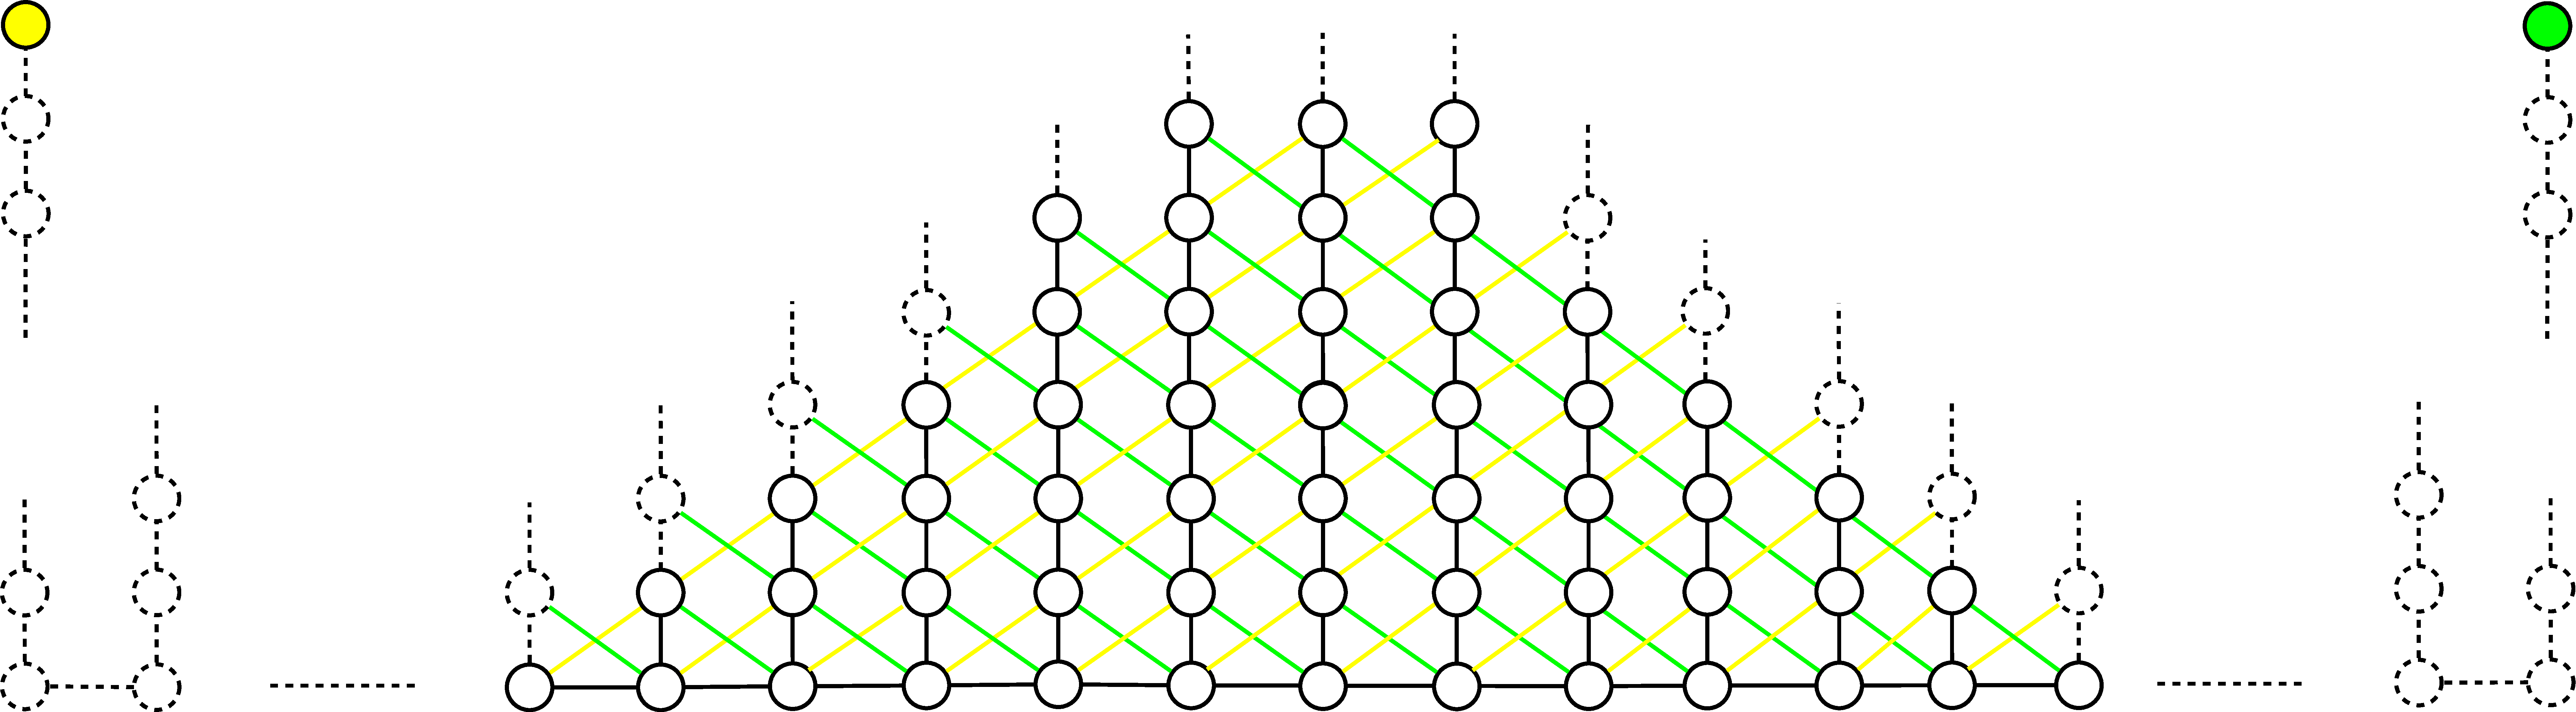
\includegraphics[width=430pt]{bilder/sonne1.pdf}
   \caption{Ein $C_{n}-Blatt$ wird durch zwei Knoten getrennt}
  	 \end{figure}
  	 
  	 \begin{figure}[h!]
		\centering
 		 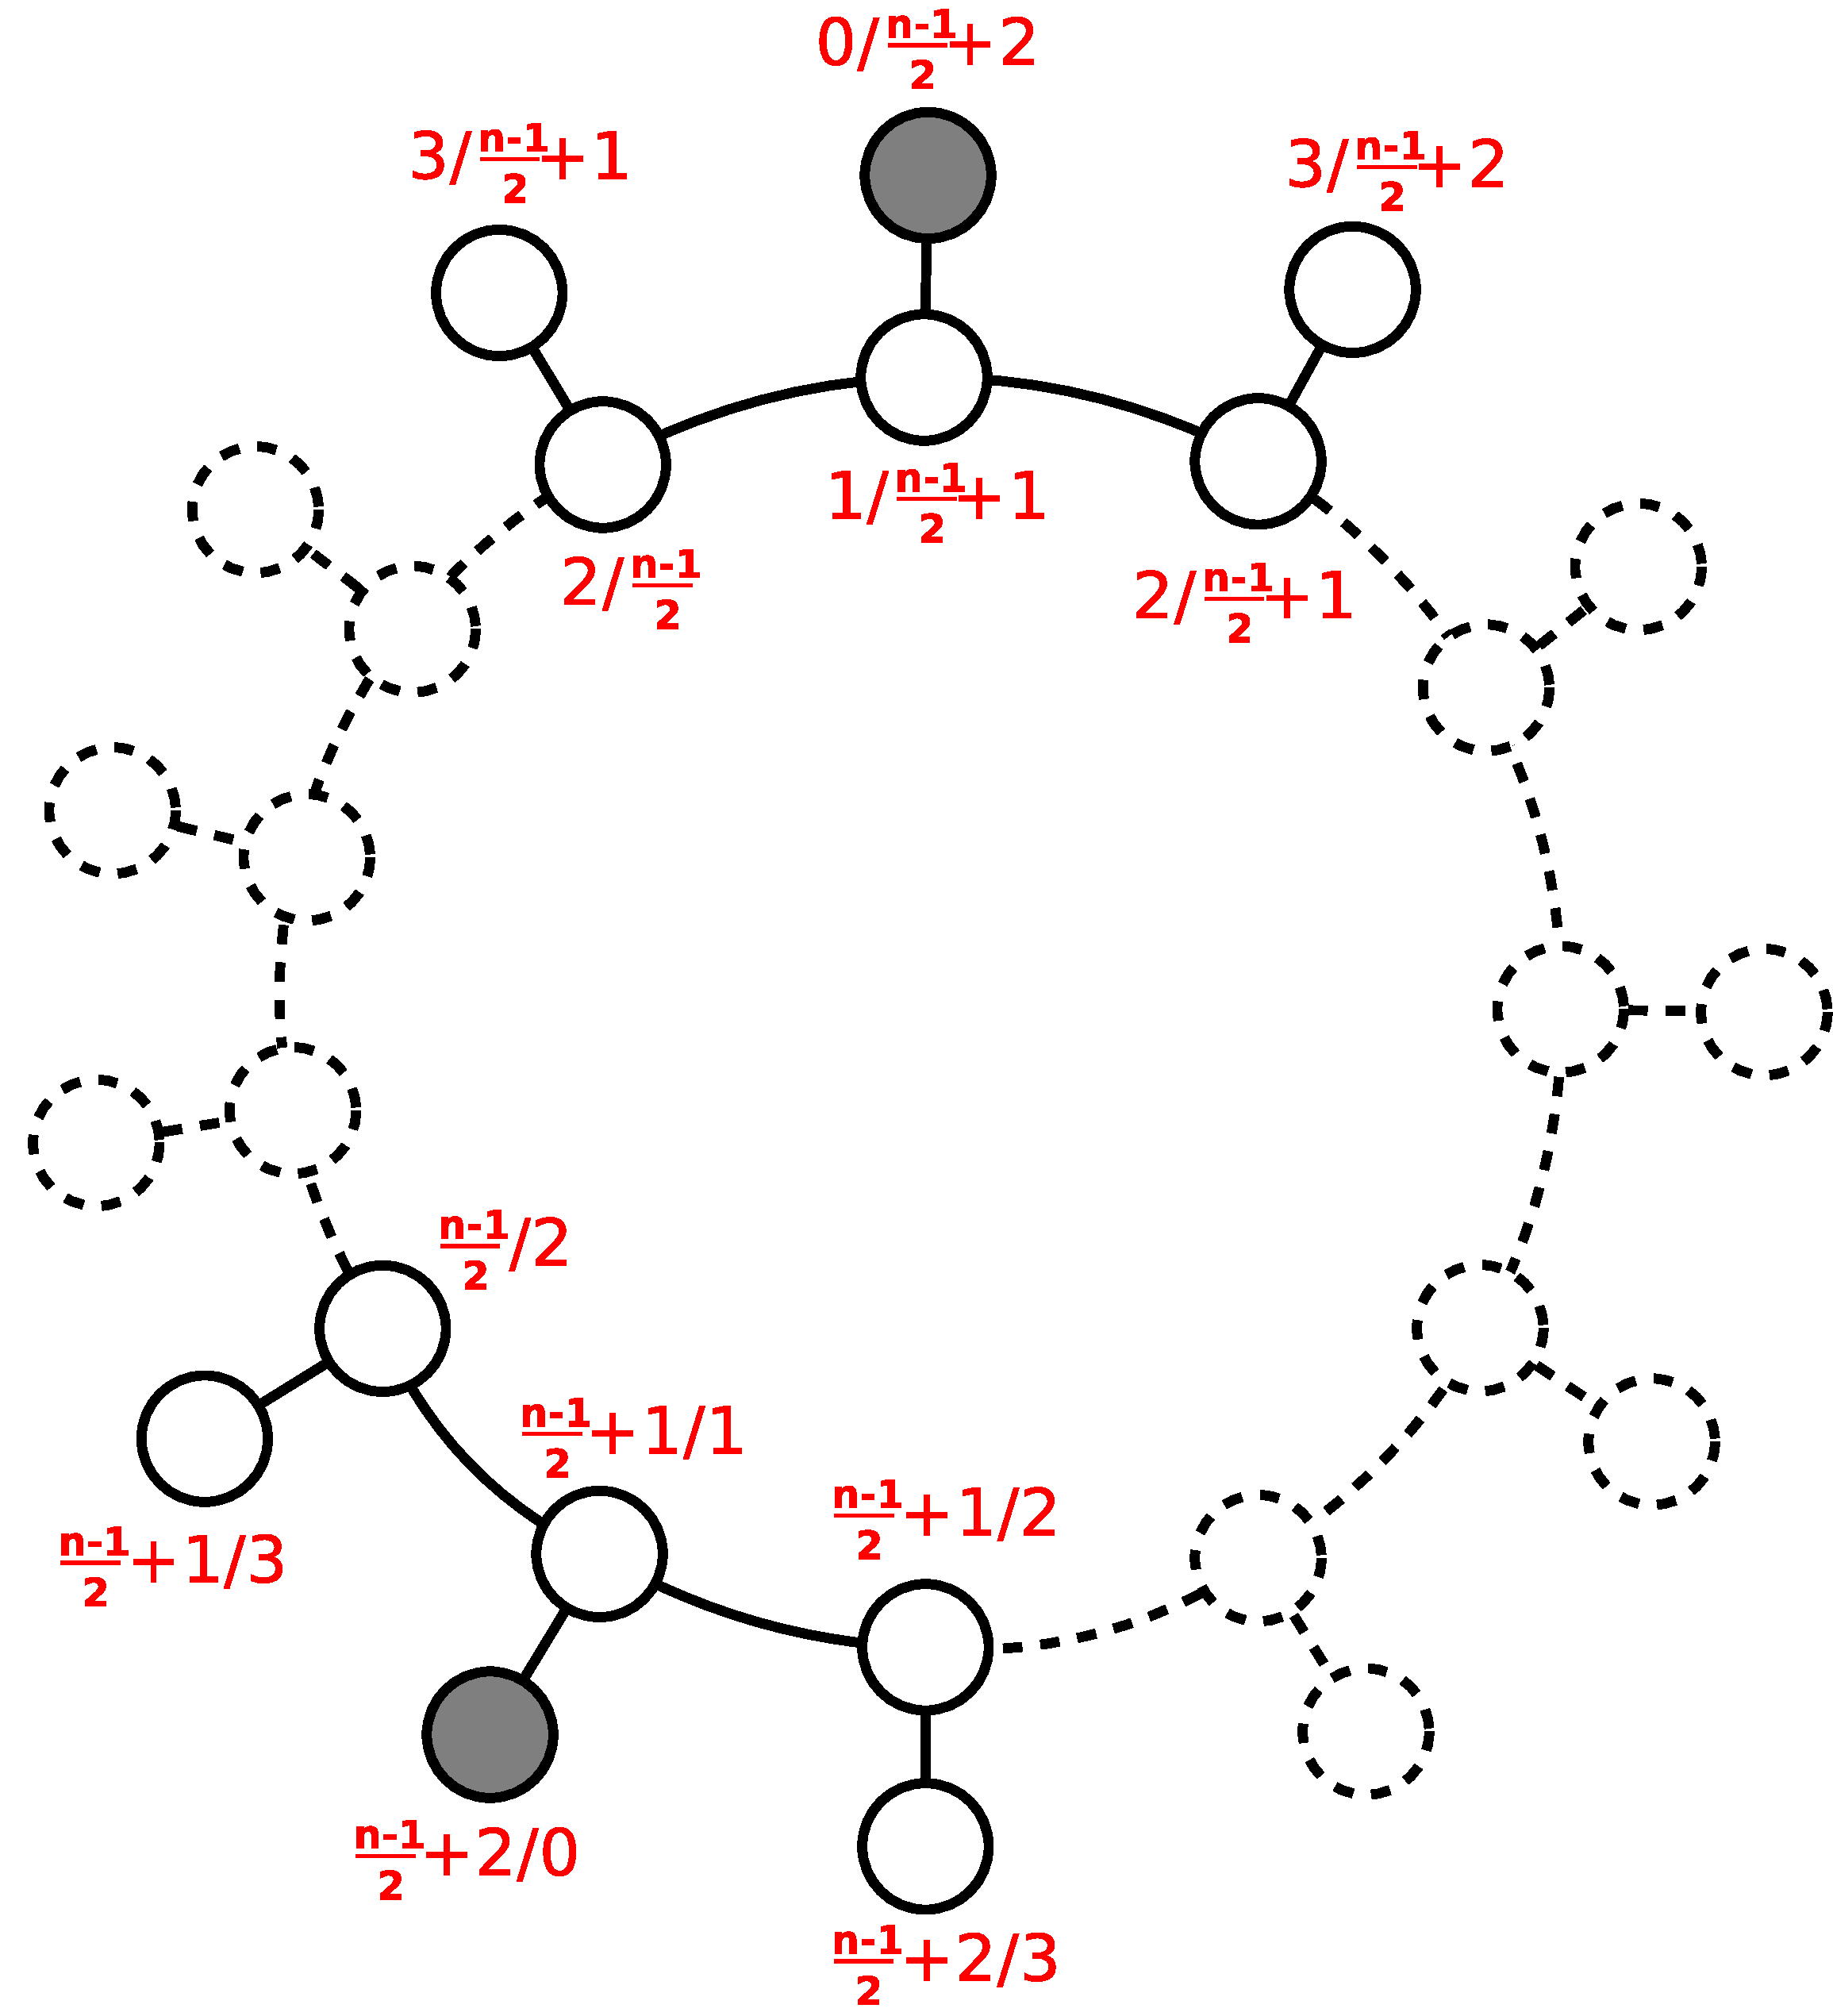
\includegraphics[width=300pt]{bilder/sonne2.pdf}
   \caption{Der Sonnengraph $S_{2n,k}$}
  	 \end{figure}
Jeder Knoten auf einem Strahl hat eine $a+x/b+x$ Markierung mit $0 \leq x \leq k$ und $a/b$ die Markierung vom Strahlursprung auf dem Kreis $C_n$.
\end{proof}  	 
\begin{defi}{\textbf{(Unvollstängiger Sonnengraph $S'_{n,k}$)}}\\
\emph{Sei ein Kreis $C_n$ für $n \geq 3$ mit der Knotenmenge $|V|=\{ c_1, \ldots , c_n \}$ und $n'$ Weggraphen $P_{k'}$ mit $1 \leq n' \leq n$ für $2 \leq k' \geq k-1$ gegeben. Die Knoten mit Grad eins auf dem $i-$ten Weg werden als $v_{i,1}$ 
und $v_{i,k-1}$ bezeichnet. Durch das Hinzufügen von $n'$ neuen Kanten der Form $\{v_{i,1},c_i\}$\\für $1 \leq i \leq n$ ensteht der zusammenhängende Sonnengraph $S'_{n',k'}$.\\
Alle als $v_{i,k-1}$ bezeichneten Knoten werden Endknoten genannt, als $c_i$ bezeichneten Knoten werden Ursprungsknoten genannt und eine Knotenmenge mit den\\Knoten $\{c_i,v_{i,1}, \ldots ,v_{i,k-1}\}$ für $1 \leq i \leq n$ als Strahl. (vgl. Abbildung \ref{bild:sonnengraph})\\
Für $n=1$ ist der Graph der Drachengraph aus \cite{blabla}.}
\end{defi}
%%%%%%%%%%%%%%%%%%%%%%%%%%%%%%%%%%%%%%%%%%%%%%%%%%%%%%%%%%%%%%%%%%%%%%%%%%%%%%%%%%%%%%%%%%%%%%%%%%%%%%%%%%%%%%%%%%%%%%%%%%%%%%%%
\subsection{Erweiterungen der Radgraphen $W_{1,i,n}$ und $W_{1,n,i}$}
Zwei ähnliche Graphklassen scheinen die Sterne $S_{1,n}$ und die Räder $W_{1,n}$ am Anfang zu sein. Doch ihre Ergebnisse bezüglich der metrischen Dimension sind kernunterschiedlich. Zunächst einmal ist die Eigenschaft nürzlich, dass jeder Sterngraph $S_{1,n}$ ein Teilgraph von dem Radgraphen $W_{1,n}$ ist mit der Eigenschaft, dass die metrische Dimension vom Stern um einiges größer ist, als von dem Rad. (Vergleiche dazu Lemma \ref{sternrad})\\
Interessant ist aber auch die Eignschaft, dass die Erweiterungen vom Stern, die gleiche Dimension haben wie der Stern selbst. Erweitert man beliebig den Graphen beliebig, so bleibt die metrische Dimension gleich. Der Beweis dafür folgt unmittelbar aus dem Satz \ref{trennungsknoten}.\\
Ganz anders ist die Situation bei den Radraphen. Dieses Kapitel widmet sich der Berechnung der metrischen Dimension von erweiterten Radgraphen. Man betrachtet dabei sowohl Erweiterung auf dem äußeren Kreis, wie auch die Erweiterungen zum inneren Knoten.\\
\clearpage
%%%%%%%%%%%%%%%%%%%%%%%%%%%%%%%%%%%%%%%%%%%%%%%%%%%%%%%%%%%%%%%%%%%%%%%%%%%%%%%%%%%%%%%%%%%%%%%%%%%%%%%%%%%%%%%%%%%%%%%%%%%%%%%%
\subsection{Der Kaktusgraph}
\begin{defi}
Als Kaktusgraph wird ein Graph genau dann bezeichnet, wenn alle seine Kreise paarweise kantendisjunkt sind, sich also höchstens einen gemeinsamen Knoten teilen.
\end{defi}
Damit sind alle Graphen mit höchstens einem Kreis Kaktusgraphen. Außerdem ist jeder Kaktusgraph außenplanar. Dadurch existiert ein polynomialzeit Algorithmus zur Berechnungin der metrischen Dimension, welcher in dem Kapitel \ref{} erläutert wird. Durch die spezifische Struktur lässt sich die metrische Dimension sogar in Linearzeit berechnen, durch den Algorithmus \ref{}.

\clearpage
%%%%%%%%%%%%%%%%%%%%%%%%%%%%%%%%%%%%%%%%%%%%%%%%%%%%%%%%%%%%%%%%%%%%%%%%%%%%%%%%%%%%%%%%%%%%%%%%%%%%%%%%%%%%%%%%
%%%%%%%%%%%%%%%%%%%%%%%%%%%%%%%%%%%%%%%%%%%%%%%%%%%%%%%%%%%%%%%%%%%%%%%%%%%%%%%%%%%%%%%%%%%%%%%%%%%%%%%%%%%%%%%%
%%%%%%%%%%%%%%%%%%%%%%%%%%%%%%%%%%%%%%%%%%%%%%%%%%%%%%%%%%%%%%%%%%%%%%%%%%%%%%%%%%%%%%%%%%%%%%%%%%%%%%%%%%%%%%%%
%%%%%%%%%%%%%%%%%%%%%%%%%%%%%%%%%%%%%%%%%%%%%%%%%%%%%%%%%%%%%%%%%%%%%%%%%%%%%%%%%%%%%%%%%%%%%%%%%%%%%%%%%%%%%%%%
\section{Metrische Dimension von $C_j-Bäumen$}
In diesem Kapitel wird eine neue Graphklasse eingeführt. Es sind Bäume mit der Eigenschaft, dass Knoten mit größerem Grad als zwei durch Kreise ersetzt werden. Das Kapitel widmet sich der Bestimmung der metrischen Dimension solcher Graphen sowie dem Vergleich der metrischen Dimension von den ursprünglichen Bäumen gegenüber den mit den Kreisen erweiterten. Zunächst fangen wir mit einem Spezialfall von solchen Graphen, den $C_3-Bäumen$, an.
\subsection{Metrische Dimension von $C_3-Bäumen$}
\begin{defi}
\label{C_{3} tree}
Für einen gegebenen Baum $T=(V,E)$ mit $deg(v_i)\leq 3$ für $v_i \in V$. Sei $$V'=\{v_k|v_k \in V \wedge deg(v_k)=3\}\subseteq V$$ eine Teilmenge der Knoten von dem Graphen $T$. Ersetze jedes Element $v_j \in V'$ durch einen $C_3$ (diese Teilgraphen werden als \emph{$C_{3,j}$} bezeichnet), so dass jeder Knoten vom $C_{3,j}$ mit genau einem Nachbarn von $v_j$ verbunden wird. Die drei Nachbarn vom $C_{3,j}$ werden als \emph{$C_{3,j}-Kinder$} bezeichnet. Sofern zwei von den $C_{3,j}-Kinder$ Blätter sind, so bezeichnet man den Teilgraphen mit dem $C_{3,j}$ und seinen Nachbarn als \emph{$C_{3}-Blatt$}. Da der entstandene Graph nur Kreise der Länge drei beinhaltet, wird er als \emph{$C_3-Baum$} bezeichnet. 
   \end{defi}
Die $C_3-Bäume$ bestehen nur aus Knoten vom Grad eins, zwei und drei, außerdem haben die einzigen Kreise, die diese Graphen beinhalten, die Länge drei. Dies bedeutet insbesondere, dass alle Knotenpaare, die nicht Teil des gleichen $C_3,j$ sind, einen eindeutigen Weg haben. Das macht jeden Knoten vom Grad zwei zu einem Trennungsknoten. Damit können diese Knoten für die Berechnung der metrischen Dimension in dem Graphen kontrahiert werden nach Satz \ref{sepvertex}.
\begin{bsp} \textcolor{white}{lala} \vspace{-6mm}
\begin{figure}[h!]
		\centering 		 
   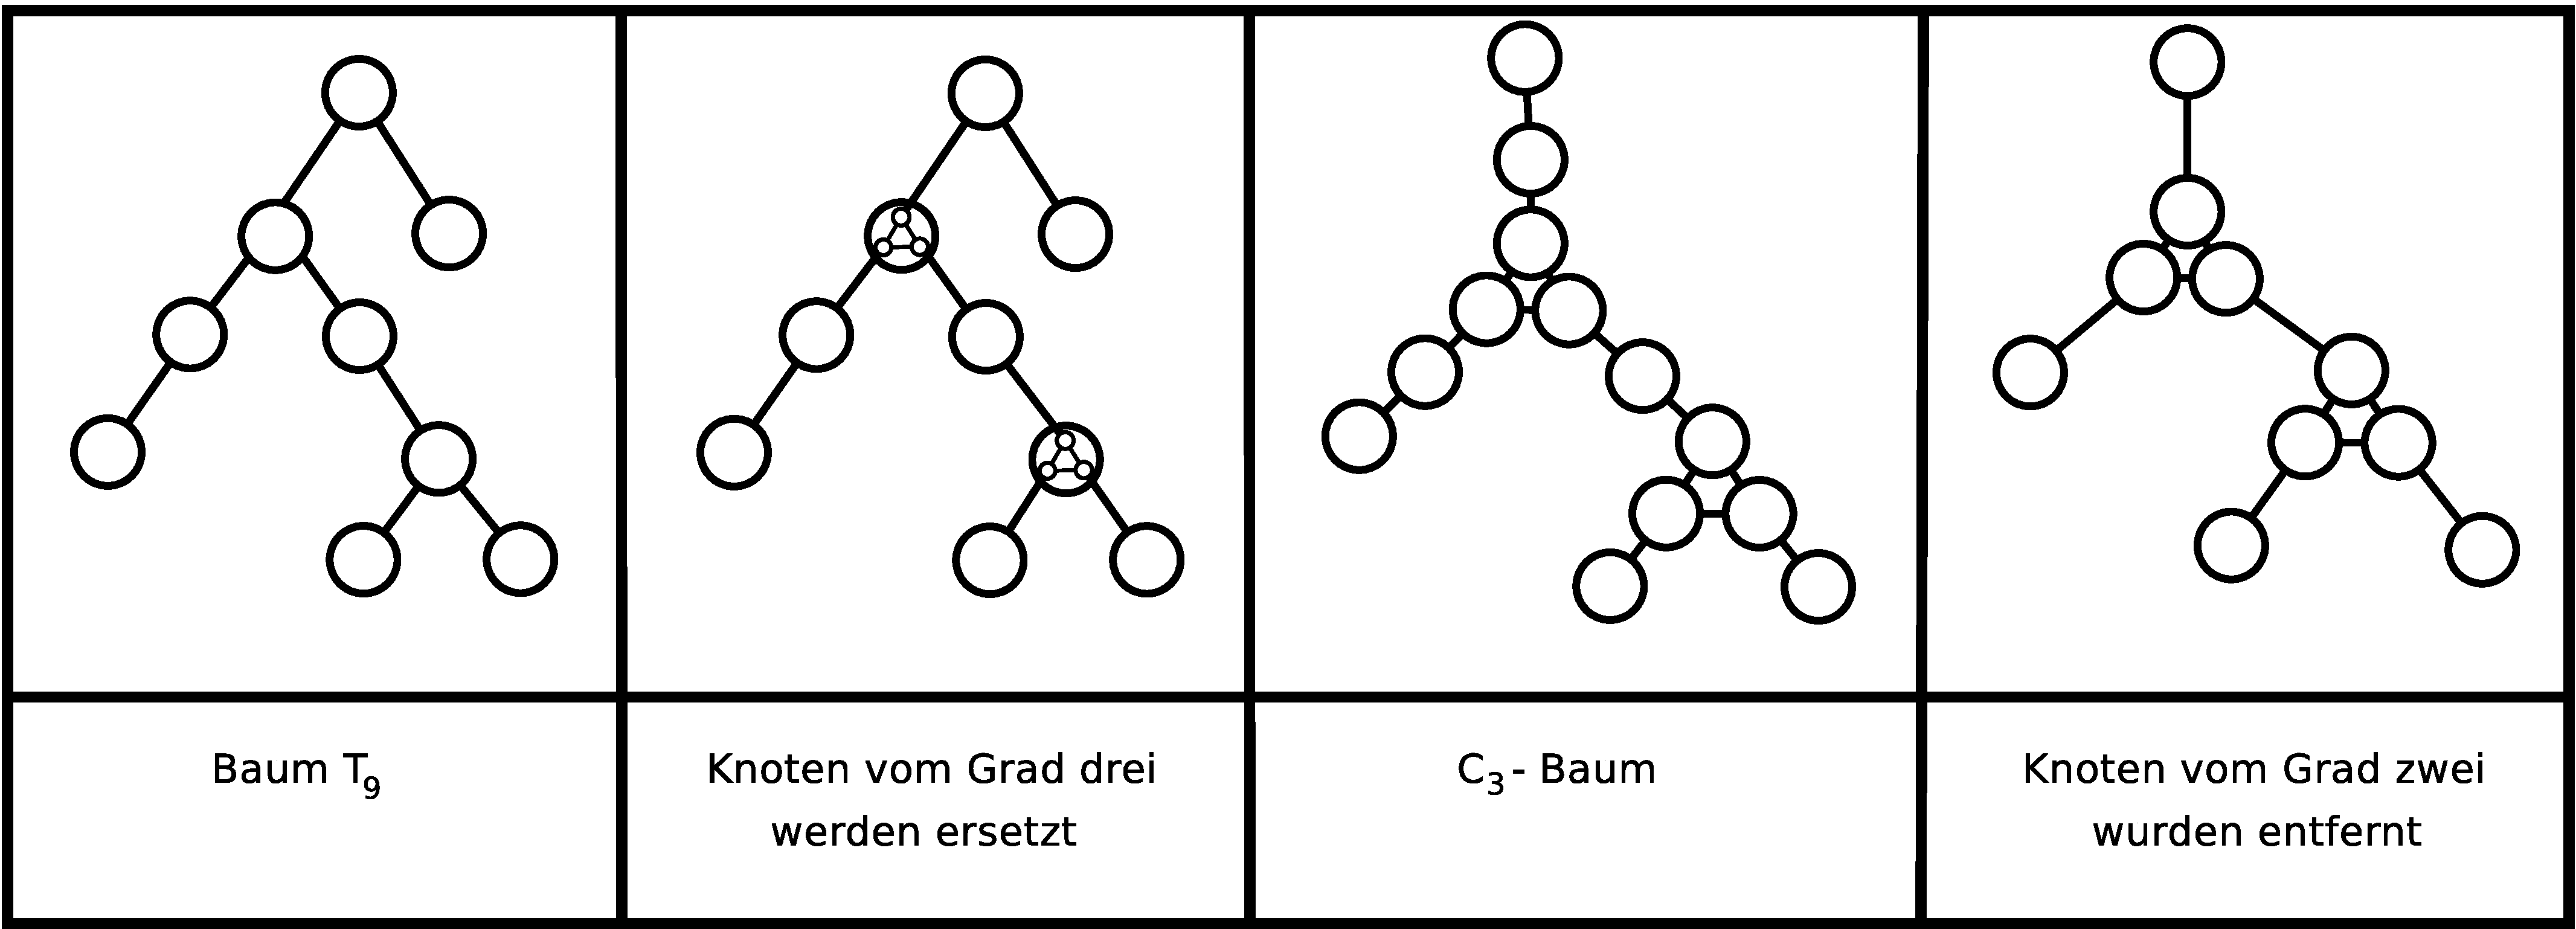
\includegraphics[width=420pt]{bilder/trees.pdf}
	\caption{Entwicklung von einem Baum zum $C_{3}-Baum$ und anschließender Knotenkontraktion}
  	 \end{figure}
\end{bsp}
Gegeben sei der abgebildete Baum $T_9$ mit neun Knoten. Dieser Baum enthält zwei Knoten von Grad drei, welche jeweils wie in der Definition beschrieben durch einen $C_3$ ersetzt werden. Um die Berechnung der metrischen Dimension des enstandenen Graphen zu erleichtern, werden alle Knoten vom Grad zwei kontrahiert.
Die metrische Dimension eines Graphen $G$ mit mindestens zwei $C_{3,j}$ ist gleich der Anzahl von seiner $C_{3}-Blätter$.
\begin{lem}
Sei $C_{3,j}$ ein beliebiges $C_{3}-Blatt$. Jede metrische Basis muss mindestens eine der folgenden Knoten $\{v_{j,1},v_{j,2},v_{j,3},v_{j,4}\}$ beinhalten.
\end{lem}
\begin{proof}[Beweis:]
\textcolor{white}{lala}
\begin{floatingfigure}[l]{200pt}
\centering
\includegraphics*[width = 100pt]{bilder/beweis.pdf}
\caption{Ein markiertes $C_{3}-Blatt$}
\end{floatingfigure}
Angenommen keiner dieser Knoten ist\\in der metrischen Basis. Durch die eindeutige Verbindung zu dem Restgraphen, welche über einen Trennungsknoten läuft, folgt aus\\Symmetriegründen dass die Knoten $v_{j,3}$ und $v_{j,4}$, sowie $v_{j,1}$ und $v_{j,2}$ identische Markierungen haben.\\Dies ist ein Widerspruch zu der Definition einer metrischen Basis.\\
Damit ist die metrische Dimension eines Graphens $G$ mit mindestens zwei $C_{3,j}$\\mindestens gleich der Anzahl von seinen $C_{3}-Blätter$.\textcolor{white}{lala}\\\textcolor{white}{lala}
\end{proof}
\textcolor{white}{lala} \vspace{-6mm}
\begin{lem}
Die metrische Dimension (MD) eines Graphen $G$ mit mindestens zwei $C_{3,j}$ ist nicht größer als die Anzahl seiner $C_{3}-Blätter$. 
\end{lem}
\textcolor{white}{lala} \vspace{-6mm}
%Um diese Eigenschaft zu beweisen werden zwei Sätze über die Struktur solcher $C_{3}-$$Bäume$ benötigt.
\begin{lem}
\label{bkb}
Jeder Knoten eines $C_{3}-Baumes$, welcher kein Blatt ist, ist ein Trennungsknoten.
\end{lem}


\begin{proof}[Beweis:]
Angenommen es gibt einen Knoten $u$, welcher kein Blatt ist und kein Trenunngsknoten. Da der Graph nur aus Knoten von Grad drei und Grad eins besteht ist der Knotengrad von $u$ drei. Dies bedeutet $u$ hat genau drei Nachbaren $v,w,x$. Da
der Knoten $u$ nach Annahme kein Trennungsknoten ist, gibt es einen Weg zwischen jedem Paar seiner Nachbarknoten.
\begin{itemize}
\item Fall I: Ein Nachbarknoten ist ein Blatt.\\ Es kommt direkt zum Widerspruch, da durch das Löschen von $u$ sich der Knotengrad von dem Blatt um eins verkleinert und damit null wird, also ein getrennter einzelner Knoten ist.
\item Fall II: Alle Nachbarknoten haben den Grad drei.\\
Es muss immernoch einen Weg zwischen jedem Knotenpaar geben damit der Graph zusammenhängend ist. Somit gibt es auch einen Weg über alle drei Knoten, sei der Anfangsknoten von diesem Weg o.B.d.A. der Knoten $v$, der Endknoten o.B.d.A. der Knoten $x$ und die Länge dieses Weges ist zwangsläufig mindestens drei. Wird wieder der entfernte Knoten $u$ betrachtet so folgt, dass der Graph einen Kreis beinhaltet welcher aus dem Weg von $v$ zu $x$ besteht und über den entfernten Knoten $u$ zurück zum Knoten $v$ geht.\\
Damit gibt es in dem Graphen mind. einen Kreis mit einer echt größeren Länge als drei und dies ist ein Widerspruch zur Definition des $C_{3}-Baumes$, welche nur Kreise der Länge drei erlaubt.
\end{itemize}
\end{proof}
\begin{lem}
\label{bkb2}
In jedem Teilgraphen eines $C_{3}-Baumes$ mit mindestens vier Knoten ist mindestens ein Knoten aus der metrischen Basis.
\end{lem}
\begin{proof}[Beweis:]
Der kleinste Teilgraph der durch das Löschen eines Knotens entstehen kann ist ein Blatt. Dieser besteht allerdings nur aus einem Knoten. Der nächstgrößere Teilgraph der durch das Löschen eines Knotens entstehen kann beinhaltet vier Knoten,genauer den unteren Teil eines $C_{3}-Blattes$. Damit beinhaltet er auch sein linkes Blatt, welches in die metrische Basis aufgenommen wird. Jeder größere Teilgraph beinhaltet diese vier Knoten. %Unabhängig davon welcher Knoten als Wurzel verwendet wurde, galt bei dem ursprünglichen Baum dass der Knoten mit der weitesten Entfernung von der Wurzel(der Knoten davor), hatte genau zwei Kinder und aus dem wurde ein $C_{3,j}-$$Blatt$.  
\end{proof}
\begin{proof}[Beweis von Lemma 27:]
Der gesamte Graph besteht nur aus Knoten vom Grad drei oder Grad eins. In die metrische Basis wird das linke Blatt von jedem $C_{3}-Blatt$ aufgenommen. Sei $n$ die Anzahl der $C_{3}-Blätter$ und $m$ die Anzahl der $C_{3,j}$, die keine $C_{3}-Blätter$ sind und bei diesem Beweis als einfache $C_{3,j}$ bezeichnet werden.
\begin{itemize}
\item Fall I. Die Knoten $u$ und $v$ haben unterschiedliche Distanzen vom Knoten $r_1$ aus der metrischen Basis. Der Knoten $r_1$ trennt die Knoten $u$ und $v$.
\item Fall II. Die Knoten $u$ und $v$ haben die gleiche Distanz vom Knoten $r_1$ aus der metrischen Basis und die Knoten $u$ und $v$ liegen im selben $C_{3,j}$.\\
O.B.d.A. sei $b_1$ der ausgewählte Knoten $r_1$ oder $b_1$ auf allen kürzesten Wegen von dem Knoten $r_1$ zu jedem Knoten in dem $C_{3,j}$. Es gibt zwei nicht getrennte Knotenpaare durch den Knoten $r_1$, das Knotenpaar $\{b_2,b_3\}$ oder das Knotenpaar $\{c_2,c_3\}$.\\
Angenommen $b_2$ und $b_3$ sind Blätter (daraus folgt das $b_1$ kein Blatt sein kann), so wird o.B.d.A. $b_3$ in die metrische Basis aufgenommen und so ist seine Markierung o.B.d.A. an der ersten Position $0$ und er ist der einzige Knoten mit dieser Markierung. Sein einziger Nachbar $c_3$, bekommt die Markierung $1$ an der ersten Position, damit ist dieser Knoten auch eindeutig markiert. Die anderen zwei Knoten $c_1$ und $c_2$ auf dem $C_3$ bekommen die Markierung $2$ an der ersten Position und ihre zwei Nachbaren $b_1$ und $b_2$, die Markierung $3$ an der ersten Position. Somit kriegen die Knotenpaare $b_2$ und $b_3$ und $c_2$ und $c_3$ unterschiedliche Markierungen und sind getrennt.\\ 	 
Sei nun $b_3$ kein Blatt, damit ist er Teil eines anderen $C_{3,j}$, welcher zwei $C_{3,j}-Kinder$ besitzt. Sind beide $C_{3,j}-Kinder$ keine Blätter, so sind sie Teile eines anderen $C_{3,j}$. Damit ist $b_3$ nach Satz \ref{bkb} ein Trennungsknoten. Der Graph ohne die Knoten $b_1$ und $b_2$ beinhaltet mindestens vier Knoten, die anderen Knoten auf diesem $C_{3,j}$ und ihre zwei $C_{3,j}-Kinder$ und nach Satz \ref{bkb2} mindestens ein Element aus der metrischen Basis.\\
Da der Knoten $b_3$ ein Trennungsknoten ist, ist die Distanz von diesem Knoten zu $b_3$ ist echt kleiner als zu jedem anderen Knoten in dem ausgewählten $C_{3,j}$. Die Markierung von $b_3$ sei o.B.d.A. an der ersten Position $a$. Sein einziger Nachbar $c_3$, bekommt die Markierung $a+1$ an der ersten Position. Die anderen zwei Knoten $c_1$ und $c_2$ auf dem $C_3$ bekommen die Markierung $a+2$ an der ersten Position und ihre zwei Nachbaren $b_1$ und $b_2$, die Markierung $a+3$ an der ersten Position. Somit kriegen die Knotenpaare $b_2$ und $b_3$ und $c_2$ und $c_3$ unterschiedliche Markierungen und sind getrennt.
\begin{figure}[h!]
		\centering
 		 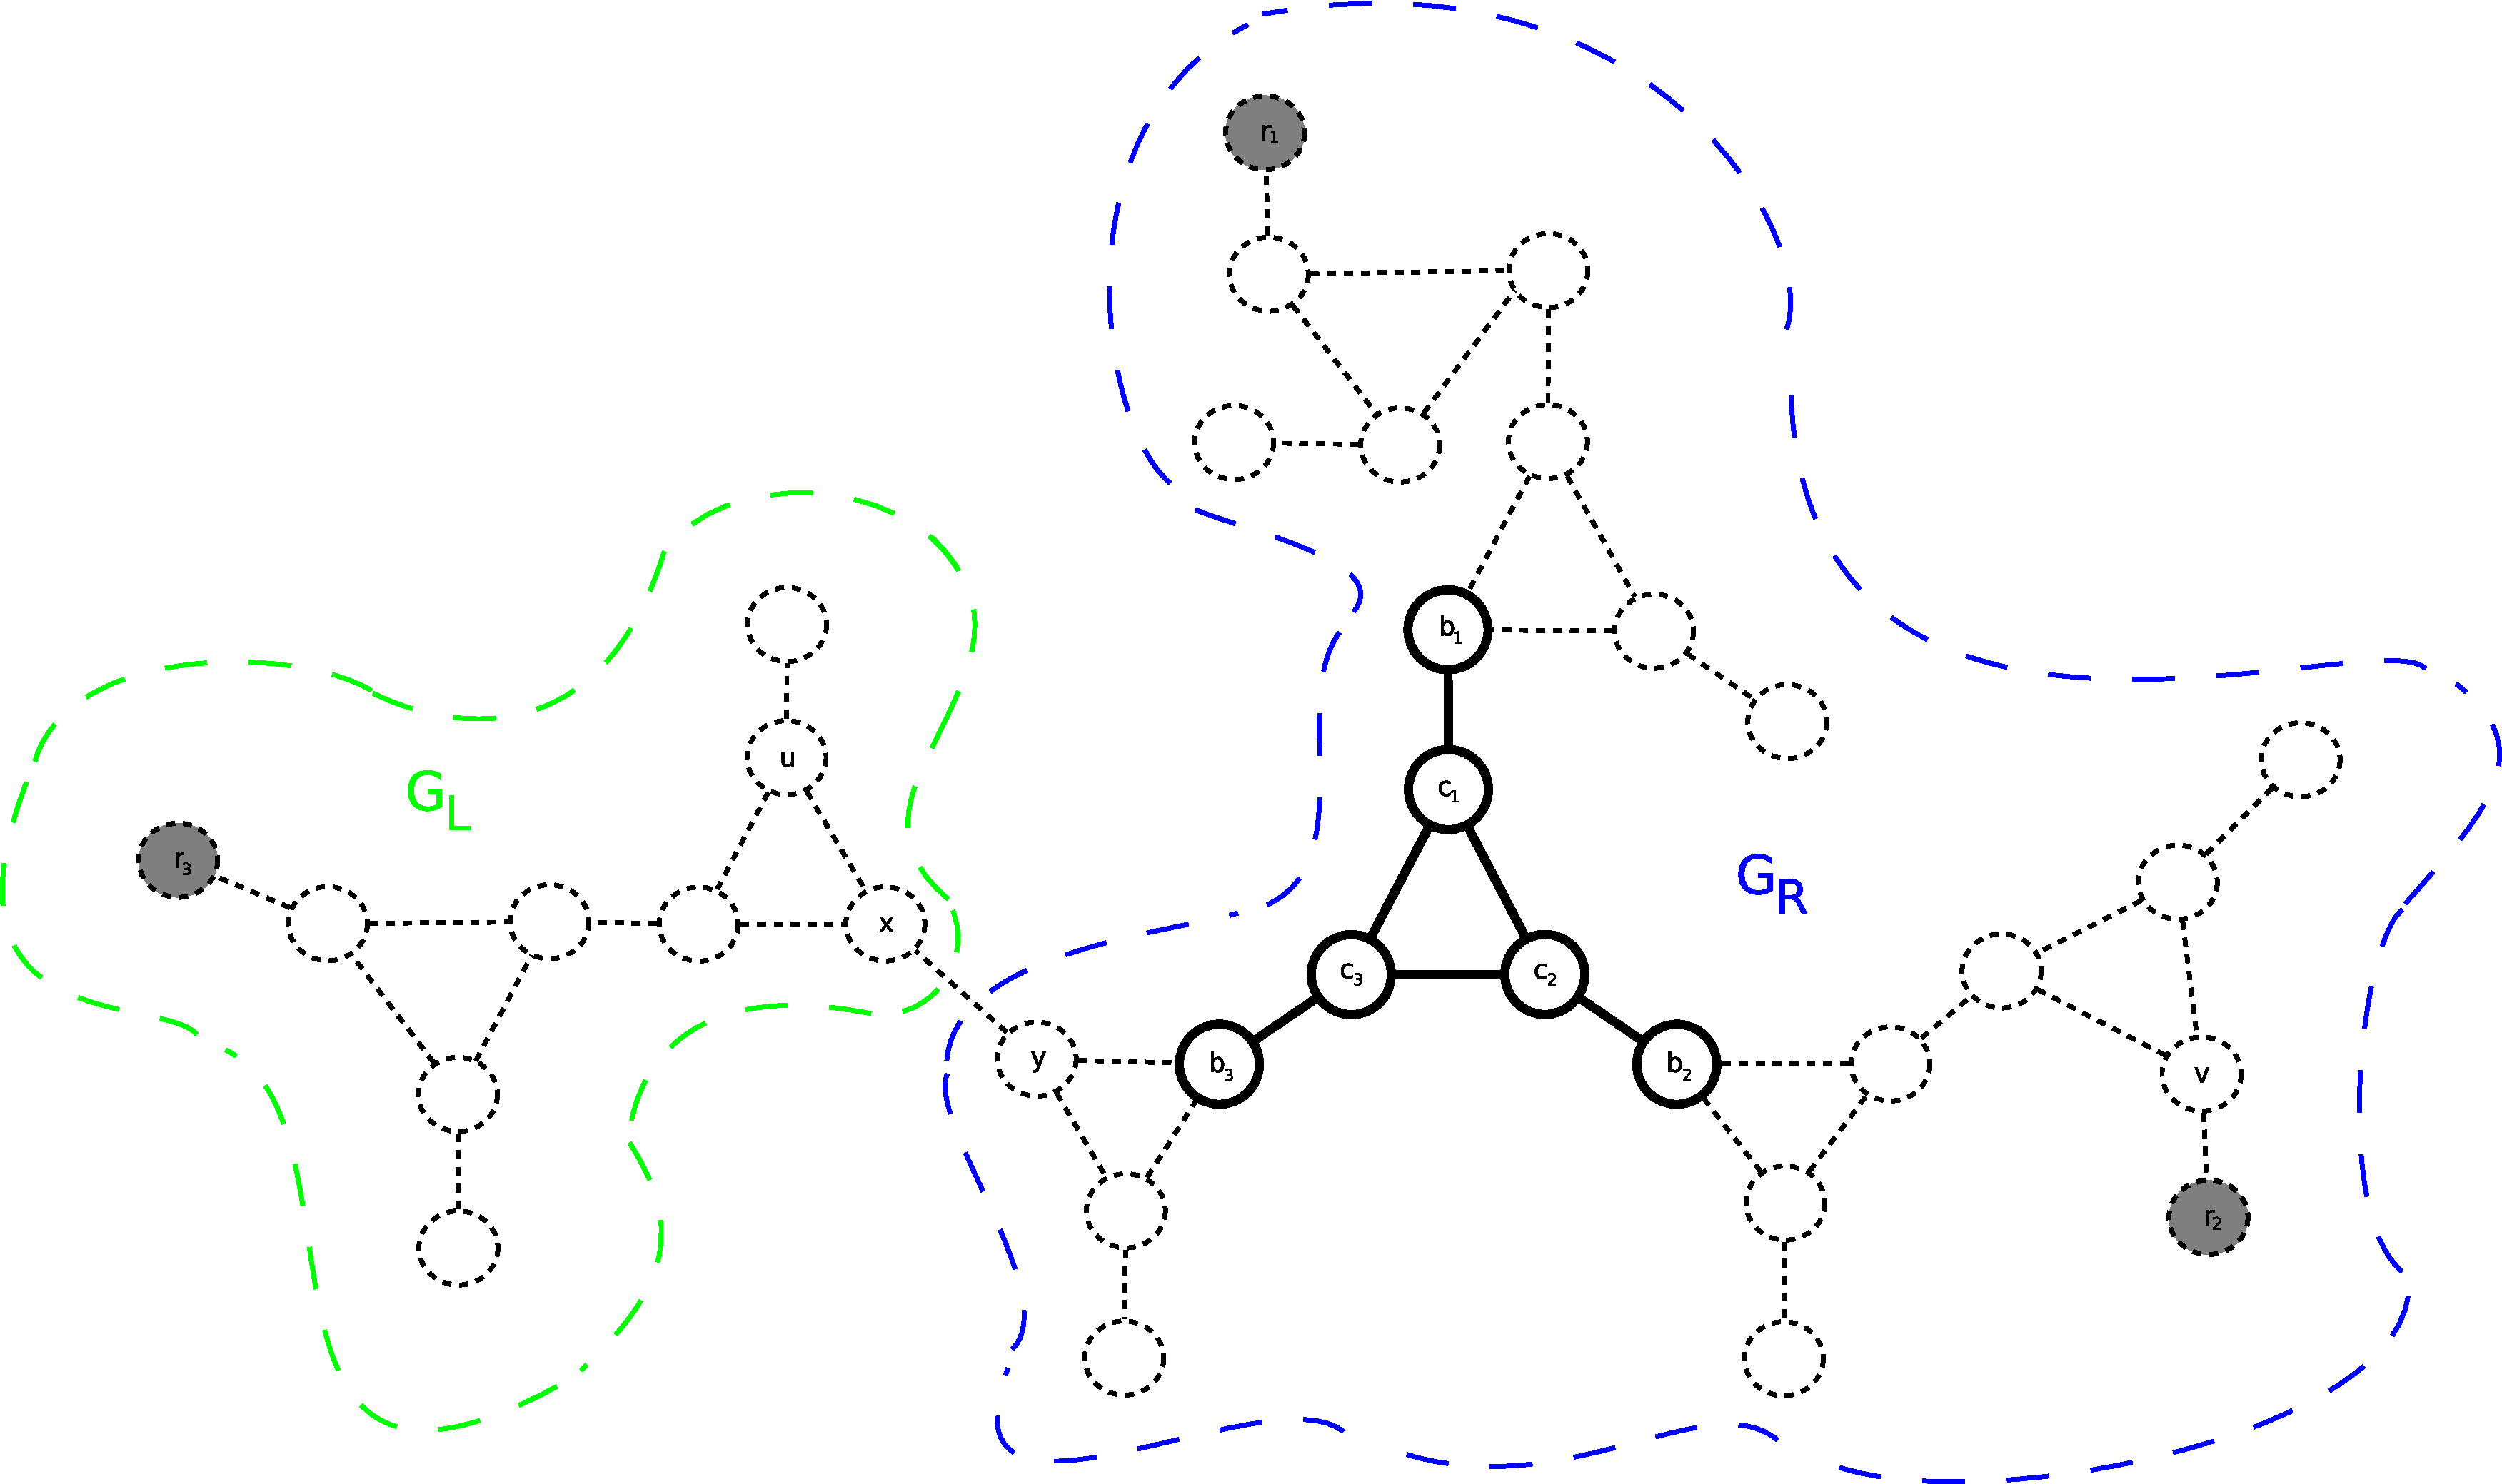
\includegraphics[width=390pt]{bilder/bew2.pdf}
   \caption{Ein Graph mit einem ausgesuchten $C_{3,j}$ und festen $r_1$, $r_2$ und $r_3$}
  	 \end{figure}

\item Fall III. Die Knoten $u$ und $v$ haben die gleiche Distanz vom Knoten $r_1$ aus der metrischen Basis und die Knoten $u$ und $v$ liegen in unterschiedlichen $C_{3,j}$.\\
Der Knoten $u$ hat entweder den Grad eins und ist ein Blatt, welches ein Nachbar eines $C_3$ ist, oder den Grad drei und ist Teil eines festen $C_{3}$. Da der Graph zusammenhängend ist, gibt es in beiden Fällen eine Kante $\{x,y\}$ in dem gleichen $C_{3,j}$ mit der Eigenschaft $x$ Teil von diesem $C_{3}$, $y$ nicht und $dist(v,y) < dist(v,x)$. Durch die zweite Anforderung kann $y$ kein Blatt sein. Nach Lemma \ref{bkb} sind $x$ und $y$ zwei Trennungsknoten, und die beiden nicht zusammenhängenden Graphen, welche durch das Entfernen des jeweiligen Knoten entstehen, haben nach Lemma \ref{bkb2} mindestens ein Element aus der metrischen Basis.\\
Der Teilgraph $G_L$ links von der Kante $\{x,y\}$ beinhaltet den Knoten $u$ und mindestens einen Knoten aus der metrischen Basis $r_3$, der Teilgraph $G_R$ an der anderen Seite der Kante $\{x,y\}$ beinhaltet den Knoten $v$ und mindestens einen Knoten aus der metrischen Basis $r_2$. Nach Satz \ref{first_theorem} sind die Knoten $u$ und $v$ getrennt.
\end{itemize}
\end{proof}
\clearpage
\begin{lem}
\textcolor{white}{x}
\begin{enumerate}
\item Fall: Der Baum besteht nur aus Knoten mit $deg(v) \leq 2$. Damit ist dieser Baum ein Weg und seine metrische Dimension ist eins.\\
\item Fall: Der Baum beinhalten genau einen Knoten mit $deg(v)=3$. Seine metrische Dimension ist zwei.
\end{enumerate}
\end{lem}

%%%%%%%%%%%%%%%%%%%%%%%%%%%%%%%%%%%%%%%%%%%%%%%%%%%%%%%%%%%%%%%%%%%%%%%%%%%%%%%%%%%%%%%%%%%%%%%%%%%%%%%%%%%%%%%%
\subsection{Verallgemeinerungen}
Unterschiedliche Möglichkeiten sind für die Verallgemeinerung von $C_3-$Bäumen möglich. Einerseits ist es möglich die Kreisordnung zu erhöhen. Eine andere Möglichkeit ist es jeden Knoten durch einen Kreis, welcher aus sovielen Knoten besteht wie der Grad des ersetzten Knotens, zu ersetzen und jeden Knoten eindeutig einem Nachbarn zuzuordnen.
\begin{comment}
\begin{defi}
For a given tree $T=(V,E)$ with $deg(v_i)\leq 3$ for $v_i \in V$, the $C_j$ Tree is build in the following way: 
   Let $$V'=\{v_k|v_k \in V \wedge deg(v_k)=3\}\subseteq V$$ be a subset of the vertices of the graph $B$. Replace each element $v_j \in V'$ by a $C_k$ with $k \geq 3$ (call this subgraphs \emph{$C_{k,3,j}$}), so that at most one vertex of $C_{k,3,j}$ is connected to exactly one neightbour of $v_j$. The three neightbours of $C_{k,3,j}$ are called the \emph{$C_{k,3,j}-$$children$}. If two of the $C_{k,3,j}-$children$ are leafs, so the subgraph including the $C_{k,3,j}$ his neighbours is called a \emph{$C_{k,3,j}-leaf$}.
\end{defi}
\begin{defi}
For a given tree $T=(V,E)$ with $deg(v_i)\leq n$ for $v_i \in V$, the $C_j$ Tree is build in the following way: 
   Let $$V'=\{v_k|v_k \in V \wedge deg(v_k)=n\}\subseteq V$$ be a subset of the vertices of the graph $B$. Replace each element $v_j \in V'$ by a $C_n$ (call this subgraphs \emph{$C_{n,j}$}), so that exactly one vertex of $C_{n,j}$ is connected to exactly one neightbour of $v_j$. The $n$ neightbours of $C_{n,j}$ are called the \emph{$C_{n,j}-$children$}. If two of the $C_{n,j}-$children$ are leafs, so the subgraph including the $C_{n,j}$ his neighbours is called a \emph{$C_{n,j}-leaf$}.
\end{defi}

\begin{defi}
For a given tree $T=(V,E)$ with $deg(v_i)\leq n$ for $v_i \in V$, the $C_j$ Tree is build in the following way: 
   Let $$V'=\{v_k|v_k \in V \wedge deg(v_k)=n\}\subseteq V$$ be a subset of the vertices of the graph $B$. Replace each element $v_j \in V'$ by a $C_k$ with $k \geq n$ (call this subgraphs \emph{$C_{k,n,j}$}), so that at most one vertex of $C_{k,n,j}$ is connected to exactly one neightbour of $v_j$. The t$n$ neightbours of $C_{k,n,j}$ are called the \emph{$C_{k,n,j}-$children$}. If two of the $C_{k,n,j}-$children$ are leafs, so the subgraph including the $C_{k,n,j}$ his neighbours is called a \emph{$C_{k,n,j}-leaf$}.
\end{defi}
\end{comment}
\begin{defi}
Sei ein Baum $T=(V,E)$ mit $deg(v_i)\leq j$ für $v_i \in V$ gegeben. Der $C_j-Baum$ resultiert daraus folgend: 
Für alle $3 \leq i \leq j$ und $i \in \mathbb{N}$ sei $$V'=\{v_k|v_k \in V \wedge deg(v_k)=i\}\subseteq V$$ eine Teilmenge der Knoten aus dem Graphen $T$. Ersetze jedes Knoten $v_n \in V'$ durch einen $C_k$ mit $k \geq i$ (bezeichnet wird dieser Teilgraph als \emph{$C_{k,i,n}$}), so dass höchstens ein Knoten von $C_{k,i,n}$ mit genau einem Nachbarn von $v_n$ verbunden ist. Die $i$ Nachbarn von $C_{k,i,n}$ werden als \emph{$C_{k,i}-Kinder$} bezeichnet. Sofern zwei dieser $C_{k,i}-Kinder$ Blätter sind wird der Teilgraph, welcher den $C_{k,i,n}$ und seine Nachbarn beinhaltet, als \emph{$C_{k,i}-Blatt$} bezeichnet.
\end{defi}

\clearpage
\begin{satz}
\end{satz}

%%%%%%%%%%%%%%%%%%%%%%%%%%%%%%%%%%%%%%%%%%%%%%%%%%%%%%%%%%%%%%%%%%%%%%%%%%%%%%%%%%%%%%%%%%%%%%%%%%%%%%%%%%%%%%%%
\subsection{Vergleich der metrischen Dimension zwischen Bäumen und $C_j-$Baümen}

%%%%%%%%%%%%%%%%%%%%%%%%%%%%%%%%%%%%%%%%%%%%%%%%%%%%%%%%%%%%%%%%%%%%%%%%%%%%%%%%%%%%%%%%%%%%%%%%%%%%%%%%%%%%%%%%
%%%%%%%%%%%%%%%%%%%%%%%%%%%%%%%%%%%%%%%%%%%%%%%%%%%%%%%%%%%%%%%%%%%%%%%%%%%%%%%%%%%%%%%%%%%%%%%%%%%%%%%%%%%%%%%%
%%%%%%%%%%%%%%%%%%%%%%%%%%%%%%%%%%%%%%%%%%%%%%%%%%%%%%%%%%%%%%%%%%%%%%%%%%%%%%%%%%%%%%%%%%%%%%%%%%%%%%%%%%%%%%%%

\section{Metrische Dimension von außenplanaren Graphen% ist in $\mathbb{P}$
}

%%%%%%%%%%%%%%%%%%%%%%%%%%%%%%%%%%%%%%%%%%%%%%%%%%%%%%%%%%%%%%%%%%%%%%%%%%%%%%%%%%%%%%%%%%%%%%%%%%%%%%%%%%%%%%%%
%%%%%%%%%%%%%%%%%%%%%%%%%%%%%%%%%%%%%%%%%%%%%%%%%%%%%%%%%%%%%%%%%%%%%%%%%%%%%%%%%%%%%%%%%%%%%%%%%%%%%%%%%%%%%%%%
%%%%%%%%%%%%%%%%%%%%%%%%%%%%%%%%%%%%%%%%%%%%%%%%%%%%%%%%%%%%%%%%%%%%%%%%%%%%%%%%%%%%%%%%%%%%%%%%%%%%%%%%%%%%%%%%
\section{Metrische Dimension von Halin Graphen} 
%%%%%%%%%%%%%%%%%%%%%%%%%%%%%%%%%%%%%%%%%%%%%%%%%%%%%%%%%%%%%%%%%%%%%%%%%%%%%%%%%%%%%%%%%%%%%%%%%%%%%%%%%%%%%%%%
%%%%%%%%%%%%%%%%%%%%%%%%%%%%%%%%%%%%%%%%%%%%%%%%%%%%%%%%%%%%%%%%%%%%%%%%%%%%%%%%%%%%%%%%%%%%%%%%%%%%%%%%%%%%%%%%
%%%%%%%%%%%%%%%%%%%%%%%%%%%%%%%%%%%%%%%%%%%%%%%%%%%%%%%%%%%%%%%%%%%%%%%%%%%%%%%%%%%%%%%%%%%%%%%%%%%%%%%%%%%%%%%%
\section{Zusammenfassung}
\begin{comment}
\begin{table}[htb]
\centering
 \renewcommand{\arraystretch}{1.5} 
\begin{tabular}{|l|c|c|c|c|c|}
\hline
$\:$Protocol & \multicolumn{1}{c|}{WSP} & GTSP & SP & SPP &SSP  \\
\hline
$\:$Cut $\&$ Choose & \Checkmark & \Checkmark  &\Checkmark & \Checkmark &  \XSolidBrush\\
\hline
$\:$Last-Diminisher & \Checkmark & (\Checkmark) & \Checkmark& \Checkmark &  \XSolidBrush\\
\hline
$\:$Lone-Chooser & \Checkmark & \Checkmark  &\Checkmark & \Checkmark &  \XSolidBrush\\
\hline
$\:$Lone-Divider & \Checkmark & \XSolidBrush  & \XSolidBrush &\XSolidBrush & \XSolidBrush \\
%\hline
%$\:$Cut your Own Piece & SPP & SP & \XSolidBrush & \Checkmark &SP& GSP \\
\hline
$\:$Divide-$\&-$Conquer & \Checkmark & \Checkmark &\Checkmark &\Checkmark &  \XSolidBrush \\
\hline
\end{tabular}
\caption{Overview: Strategyproofness of proportional cake-cutting protocols}\label{ov}
\end{table}
\end{comment}
%%%%%%%%%%%%%%%%%%%%%%%%%%%%%%%%%%%%%%%%%%%%%%%%%%%%%%%%%%%%%%%%%%%%%%%%%%%%%%%%%%%%%%%%%%%%%%%%%%%%%%%%%%%%%%%%
%%%%%%%%%%%%%%%%%%%%%%%%%%%%%%%%%%%%%%%%%%%%%%%%%%%%%%%%%%%%%%%%%%%%%%%%%%%%%%%%%%%%%%%%%%%%%%%%%%%%%%%%%%%%%%%%
%%%%%%%%%%%%%%%%%%%%%%%%%%%%%%%%%%%%%%%%%%%%%%%%%%%%%%%%%%%%%%%%%%%%%%%%%%%%%%%%%%%%%%%%%%%%%%%%%%%%%%%%%%%%%%%%
\subsection{Ähnliche Arbeiten}
\begin{comment}
\end{comment}
%%%%%%%%%%%%%%%%%%%%%%%%%%%%%%%%%%%%%%%%%%%%%%%%%%%%%%%%%%%%%%%%%%%%%%%%%%%%%%%%%%%%%%%%%%%%%%%%%%%%%%%%%%%%%%%%
%%%%%%%%%%%%%%%%%%%%%%%%%%%%%%%%%%%%%%%%%%%%%%%%%%%%%%%%%%%%%%%%%%%%%%%%%%%%%%%%%%%%%%%%%%%%%%%%%%%%%%%%%%%%%%%%
%%%%%%%%%%%%%%%%%%%%%%%%%%%%%%%%%%%%%%%%%%%%%%%%%%%%%%%%%%%%%%%%%%%%%%%%%%%%%%%%%%%%%%%%%%%%%%%%%%%%%%%%%%%%%%%%
\section{Offene Fragen und zukünftige Forschung}
\cite{res},\cite{n-3},\cite{OnDet},\cite{Bounds},\cite{Discrep},\cite{Cartesian},\cite{upper},\cite{landmarks}, \cite{Erdos}
\pagebreak

%%%%%%%%%%%%%%%%%%%%%%%%%%%%%%%%%%%%%%%%%%%%%%%%%%%%%%%%%%%%%%%%%%%%%%%%%%
%%%%%%%%%%%%%%%%%%%%%%%%%%%%%%% ENDE TEXTTEIL %%%%%%%%%%%%%%%%%%%%%%%%%%%%
%%%%%%%%%%%%%%%%%%%%%%%%%%%%%%%%%%%%%%%%%%%%%%%%%%%%%%%%%%%%%%%%%%%%%%%%%%

\clearpage
\thispagestyle{empty}
%\vspace*{\fill}g
\pagestyle{plain}
\bibliographystyle{plain}
\bibliography{references}
\thispagestyle{empty}
%\vspace*{\fill}g
\pagestyle{plain}
\clearpage

\listoffigures

\listoftables
\thispagestyle{empty}
%\pagebreak
\pagestyle{plain}
%\printindex
\end{document}
